\documentclass[12pt, a4 paper]{article}

\usepackage{My_packages}
%\usepackage[utf8]{inputenc}
%\usepackage{xcolor}

\definecolor{dg}{rgb}{0.0, 0.6, 0.1}
\newcommand{\Andrew}[1]{\textcolor{dg}{#1}}
\newcommand{\Arjen}[1]{{\color{brown}#1}}
\newcommand{\Vasu}[1]{{\color{purple}#1}}


\date{ }

\begin{document}
\iffalse
\begin{titlepage}
    Paper Rough draft
\end{titlepage}
\fi

\tableofcontents
\newpage

\section{Introduction}

% What do we know about magnetic fields?   
The origin and structure of the Galactic magnetic field remains an long standing unresolved problem in astrophysics. What is apparent, however, is the vital role it plays, especially in terms of cosmic ray propagation within the Galaxy. The incompleteness of the observational data, required to probe the Galactic magnetic field structure on many different scales, limits significantly our ability to describe cosmic ray propagation through the Galaxy. This is especially true when it comes to the modelling of cosmic ray propagation out in the Galactic halo where our knowledge of the magnetic field is particularly weak.

%  tools used to detect magnetic fields namely RM and synchrotron. And typical values for these fields
A variety of methods allow observational probes of Galactic magnetic fields, such as starlight polarisation and infrared emission from dust grains, or Zeeman splitting of spectral radio lines in the dust clouds \textcolor{blue}{\cite{Beck_2007}}. Galactic magnetic fields are also probed by Pulsar dispersion with Faraday rotation, which is sensitive to the magnetic-field component parallel to the line of sight $B_{\parallel}$, and synchrotron radiation which probes the component perpendicular to the line of sight $B_{\perp}$. A major drawback in using the Pulsar dispersion measure along with the Faraday rotation measure method for probing Galactic magnetic fields is that it relies heavily on the lines of sight along which Pulsars are found, which places a strong focus on the regions close to the Galactic plane. Therefore, this method is of most use for probing the magnetic field in the Galactic disc region, and is not so useful for probing the magnetic field out in the Galactic halo. Synchrotron radiation on the other hand is produced via the gyration of non-thermal electrons along magnetic field lines. This method can thus be used to probe magnetic fields also in the Galactic halo.

% Observations from S-PASS and Planck
With the help of the aforementioned techniques, we can estimate the strength and direction of the magnetic field in different parts of the Galaxy. 
For the Galactic halo the S-PASS observations made at 2.3 GHz seem to suggest that the field strength in the halo bubbles can be anywhere between $6-10~\mu $G depending on the proton-electron ratio. S-PASS observation however are subject to depolarisation of polarised synchrotron radiation via Faraday rotation due to its low observation frequencies and this data set is also not sensitive to a portion of the Fermi bubbles because of its positioning in the southern hemisphere. For this reason data from Planck and WMAP are more helpful when probing magnetic fields in the Galactic halo due to their all sky coverage and observation bandwidths which are not sensitive to Faraday rotation effects.

% Other magnetic field models and energies in the halo.

Several efforts have made in modelling magnetic field in the Galaxy namely by \cite{Jaffe_2010},\cite{Jaffe_2011}, \cite{Sun},and \cite{JF12}. It should be noted that our understanding for Galactic disc is much better than the halo due to larger amount of observations present. However, widely used models like JF12 have made considerable contributions also towards modelling of Galactic halo. One drawback with JF12 is that they mask out the Fermi bubble regions in their models but, S-PASS observations tell us that magnetic field strength in this region is not negligible. Therefore, it is important to consider modelling the Galactic halo including the Fermi bubbles.
\Vasu{I have rewritten this section.}
%\Arjen{I would say that this paragraph needs improving. Is the JF12 model, for example, really focussed mostly on the disc? They spent quite some effort on modelling the halo as well. And this last statement, that the fields in the halo for these models is rather weak, can that really be stated so generally for all models? A statement like that needs a bit more motivation or explanation, I would say, or perhaps it should be more specific especially for the Fermi bubbles region.}

The observations from FERMI-LAT \cite{Su_2010} in the gamma ray regime unveiled giant bipolar gamma ray bubbles extending up to $\approx$~3~kpc radially and $\approx$~8~kpc in the z-direction, having a total energy of $\approx 10^{(54-55)}$~ergs. Recently, observations from eROSITA in X-ray regime further suggest existence of even larger bubbles going up to  $\approx$~7~kpc radially and $\approx$~14~kpc in the azimuthal direction, having a total energy of $\approx 10^{(56)}$~ergs. These observations strongly motivate the requirement of a magnetic field model focusing on the halo. Henceforth, for the sake of simplicity we will address the two bubbles together as the Galactic halo bubbles.

% Short note on non-thermal electron distribution.
Apart from the Galactic magnetic field, our understanding of the non-thermal electron distribution in the Galaxy is also poor. We have some information on the distribution of cosmic ray electrons from the observations made by \Vasu{enter observation details.}\hyperlink{CR spectra}{https://arxiv.org/pdf/1108.4822.pdf} which peaks at 1GeV.
Currently, there are a few ways to model the spatial distribution of these relativistic electrons; for example, with GALPROP \cite{Hammurabi} or the analytical WMAP model \cite{WMAP_Page}. \Arjen{Perhaps this paragraph can be extended a bit. Why do we care about the non-thermal electron distribution when talking about the Galactic magnetic field? Why is our knowledge of the non-thermal electron distribution so poor? How can it be measured and how do the models that you mention relate to the measurements?} \Vasu{Currently working on it.}
However, when modelling Galactic magnetic fields, Galactic cosmic ray electrons are not the only particles of interest. 

% Importance of UHECRs
An understanding of Galactic magnetic fields is tied to an understanding of the propagation and arrival direction of extra-galactic cosmic rays (with energies higher than $\approx$~$10^{18}$), also known  as ultra high energy cosmic rays (UHECRs). These UHECRs are constituted by charged protons or nuclei, and therefore their origin directions are scrambled by the magnetic fields they pass through en-route to Earth. The paths of these UHECRs can, therefore, be drastically changed depending on the strength and geometry of the field. Different models of the Galactic magnetic field give vastly different predictions for the deflection of UHECRs (see e.g.~Ref.~\textcolor{blue}{ADD REF}). Recently, significant anisotropies in the UHECR sky have been discovered~\textcolor{blue}{REFS TO DIPOLE/STARBURST CORRELATIONS/TA HOTSPOT}. Due to the deflections in the Galactic magnetic fields, the interpretation of these results in terms of the localisation of the UHECR sources is extremely hard and hence, the knowledge of Galactic magnetic fields is extremely important. 

% Introduction to brief layout of the paper
In this paper we propose a simple toy model for the magnetic field out in the Galactic halo region which encompasses the Galactic halo bubbles. We provide a detailed explanation of the electron distribution and the toy model magnetic fields in section 2. This is followed up by the comparison of the synthetic polarised synchrotron maps and the Planck data and the uncertainty estimates on parameters in section 3. In section 4 we focus on the arrival directions of ultra high energy cosmic rays $\rm E = 30$~EeV from our toy model and discuss how the uncertainties in the parameters can propagate errors in estimating the cosmic ray directions. We also compare results from the toy model and the halo fields from JF12 model. Lastly, we talk about our deductions from this study in section 5.

\iffalse
 We rely on polarised synchrotron emissions and rotation measures, both of which are line of sight integrated components. We investigate both polarised synchrotron emission which depends on the perpendicular component of the magnetic field and the Faraday rotation measures that rely on the parallel component of the magnetic field and the thermal electron density. 
We also do an extensive study of the affects on the arrival directions of cosmic rays from our toy model and how the uncertainties in the parameters propagate uncertainties in the estimation of these directions.
Since our main focus lies in probing the magnetic field in the Galactic halo, we have cut out the region of the Galactic disc from our model. However, the affect of our toy model and JF12 disc field will also be discussed in this paper.
\fi

\section{Methodology}
\label{method}

% Toy model introduction and comparison to JF12 
\subsection{Galactic Halo Magnetic Field Model}
\label{GMF}
In this paper we motivate a toy model as means of a preliminary attempt to provide a model for the Galactic halo bubbles. We propose a simple axisymmetric torroidal field with a Kolmogorov turbulent field with a phase-space spectrum of $11/3$ given by the following expression:
\begin{equation}\label{TM_equation}
        B_{\mathrm{toy}}= B_{\rm{str}}\mathrm{e}^{{(-\abs{{z}}/Z_{{\mathrm{mag}}})}} \mathrm{e}^{{(-z_{{\mathrm{min}}}/\abs{{z}})}}\mathrm{e}^{{(-\abs{{r}}/R_{{\mathrm{mag}}})}} + B_{\rm{tur}}
\end{equation}
The structured field has 3 free parameters: $B_{\rm str}$ as the peak value of the field and $R_{\rm {mag}}$ and $Z_{\rm {mag}}$ the radial and azimuthal cut off respectively. The direction of the toroidal field is opposite above and below the Galactic plane. The visualisation of the field in XY and XZ cross-section is shown in
figure[\ref{fig:Vis_TM}]. 

We use CRPropa~3 \cite{CRPropa3_2016} for generating turbulent fields which has a power law spectrum and peak field value of $B_{\rm{tur}}$. 
The minimum and maximum values of wavelength to generate these fields are  $L_{min}$ = 200 pc and $L_{max}$ = 400 pc. For computational reasons we do not have a large difference between  $L_{min}$ and $L_{max}$.
The turbulent field thus has effectively only 1 free parameter which is the peak of value $ B_{\rm{tur}}$, the coherence length of the field is kept fixed at 150~pc for simplicity.  In appendix ~\ref{Appendix_B} we show the power-spectrum plot this field.

Since, we focus only on the Galactic latitude region of the sky which probes the Galactic halo, we do not include any disk magnetic field component in this model. 
For the purposes of comparison we used the JF12 model as it is one of the most widely known, Galactic magnetic field models.
We studied each component of the JF12 field separately in order to ascertain how the different components of the Galactic magnetic field model act individually and together. However, it should be noted that the JF12 model was motivated by observations which masked out a large part of the Galactic bubble region, and adopts magnetic fields strengths weaker than the ones suggested by S-PASS observation.% Based on observations, it is highly likely that the strength of the magnetic field in the Galactic halo is underestimated in the JF12 model. \Arjen{This statement might need a bit more clarification, it's rather strong and I don't think this is generally known/realised/accepted by everyone. Perhaps at least a mention of which observations show this is appropriate.}
% toy model cross section plots subject to the end results from equipartition scans.
\begin{figure}[h!]
    \centering
    \includegraphics[width = 8cm]{Images/toymodel_XY_6Sep.png}%
    \includegraphics[width = 8cm]{Images/toymodel_XZ_6Sep.png}
    \caption{Cross-section of toy model for the Galactic magnetic field in the Galactic halo region in the XY and XZ plane (with the Galactic plane in the XY plane at $z=0$) showing their drop in two dimensions.\Vasu{Plot will be changed after the final analysis.} }
    \label{fig:Vis_TM}
\end{figure}
\clearpage

%Discuss the electron distribution
\subsubsection{Electron Distribution}

In order to produce synthetic synchrotron maps an electron distribution is required.
The JF12 model considered both the WMAP analytical expression \ref{Eq_WMAP_EdNdE}
and simulated electron distribution from GALPROP. They used the latter for their model in their paper.
The two models are quite different. The WMAP \cite{WMAP_Page} model is an analytical expression whereas the GALPROP \cite{Hammurabi} is based on numerical simulations and the distribution of supernova remnants in the Galaxy. For our toy model we adopted the WMAP distribution model. Our current knowledge of the non-thermal electron distribution in the Galaxy, especially in the Galactic halo region, is very limited. We therefore prefer to adopt a simple analytical model in order to avoid adding further layers of complexity. The WMAP electron distribution model is:
\begin{equation}\label{Eq_WMAP_EdNdE}
    \frac{\mathrm{d}N_e}{\mathrm{dlog}E_{e}} =     C_\mathrm{norm} \left(\frac{E_e}{\rm E_{\rm 10 GeV}}\right)^{-p+1} e^{-r/R_{\mathrm{el}}} \mathrm{sech}^2(z/Z_{\mathrm{el}}) 
\end{equation}
where $\frac{\mathrm{d}N_e}{\mathrm{dlog}E_{e}}$ is the differential electron density in a certain energy bins
in units of ${\rm cm}^{-3}$, $p =3$ is the spectral index. The parameters, $C_\mathrm{norm}$, describes the 10~GeV electron density, and $R_{\mathrm{el}}$ \& $Z_{\mathrm{el}}$ describe the radial and azimuthal spatial cut-offs. 


% EdNdE plots for some arbitrary parameters which will be fixed post equipartition scans.
\begin{figure}[h!]
    \centering
    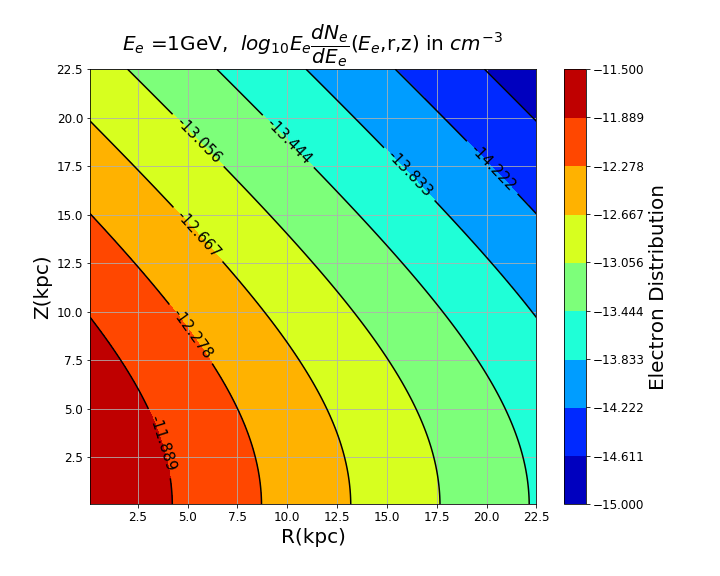
\includegraphics[width= 8cm]{Images/EdNdE_1GeV.png}%
    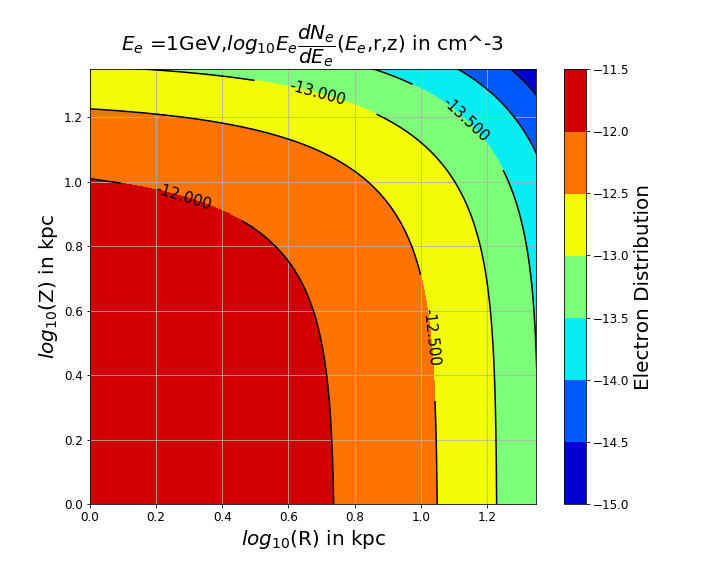
\includegraphics[width = 8cm]{Images/Logscale_EdNdE_1GeV.png}
    \caption{Electron distribution for $R_{\mathrm{el}} = 5$ kpc and $Z_{\mathrm{el}} = 10$ kpc in linear scale on left and log-scale on right. The electron distribution an exponential drop with increasing R and Z. \textcolor{purple}{Change the plot when you have new set of parameters from Equipartition results. \Andrew{units should be mentioned within log term} \Vasu{-will correct them for the final set of parameters.}}}
    \label{fig:my_label}
\end{figure}

% synchrotron radiation expressions and theory, also the appendix.
\subsection{Synchrotron Emission}\label{Synchrotron_theory}

\subsubsection{Intensity \& polarisation}
Synchrotron radiation or magneto-bremsstrahlung radiation is the radiation produced due to charged particles that gyrate at relativistic speeds around a static magnetic field. The radiation produced via synchrotron is often linearly polarised.
%The radiation received from a single particle is elliptically polarised and the sense of polarisation (right or left handed) is determined by whether the line of sight sits inside or outside the cone of radiation.
%However, for a distribution of particles that vary smoothly with the pitch angle, the elliptical component cancels out and so the emission cones will contribute equally on each side of the line of sight. The radiation then is linearly polarised. 
The polarised emission can be visualised as an ellipse where the major axis is the perpendicular component ($J_{\rm \perp}$) and the minor axis is the parallel ($J_{\parallel}$) component. We provide a detailed explanation of this in appendix~(\ref{Appendix_A}). 

Equations \ref{Jperp} and \ref{Jpara} describe the two polarised components $J_{\perp}$ and $J_{\parallel}$ for a  given peak photon energy $E_{\gamma}^{\mathrm{peak}}$. In this case, $E_{\gamma}^{\mathrm{peak}} = 1.175 \times 10^{-4}$ eV which is corresponding 28.4 GHz, the peak frequency for 30 GHz Planck data.
\begin{equation}\label{Jperp}
 {J_{\perp}^l} =   \int_{\mathrm{log}E_e^{\mathrm{min}}}^{\mathrm{log}E_e^{\mathrm{max}}}\mathrm{dlog}E_{e} \  \frac{\mathrm{d}N_e}{\mathrm{dlog}E_{e}} \  \left[F\left(\frac{E_{\gamma}}{E_{\gamma}^{\mathrm{peak}}}\right) + G\left(\frac{E_{\gamma}}{E_{\gamma}^{\mathrm{peak}}}\right)\right] * \frac{B_{\perp}}{B_{\mathrm{crit}}}\frac{m_{e}}{h} \frac{8\pi \alpha}{9} 
\end{equation}

and,

\begin{equation}\label{Jpara}
{J_{\parallel}^l} = \int_{\mathrm{log}E_e^{\mathrm{min}}}^{\mathrm{log}E_e^{\mathrm{max}}}\mathrm{dlog}E_{e} \ \frac{\mathrm{d}N_e}{\mathrm{dlog}E_{e}} \  \left[F\left(\frac{E_{\gamma}}{E_{\gamma}^{\mathrm{peak}}}\right) - G\left(\frac{E_{\gamma}}{E_{\gamma}^{\mathrm{peak}}}\right)\right] * \frac{B_{\perp}}{B_{\mathrm{crit}}}\frac{m_{e}}{h} \frac{8\pi \alpha}{9}
\end{equation}
where the functions,
\begin{align}
F(x) = x \int_x^\infty K_{5/3}(x') dx',  \hspace{1cm}  \&   G(x) = x K_{2/3}.
\end{align}
$B_{\mathrm{crit}} \frac{m_e^2c^3}{e\hbar} = 4.414 \times 10^{13}$~G is defined as the critical magnetic field, $m_e = 0.511$ MeV is the mass of electron , $h = 4.136 \times 10^{-15}$~eV-sec is the Planck's constant and $\alpha \approx \frac{1}{137}$ is the fine structure constant.

For clarity, several of the conventions are noted. The parallel component of polarisation (${J_{\parallel}}$) is orientated in the same direction as  $\vec{B_{\perp}}$, and the perpendicular component of polarisation (${J_{\perp}}$) is perpendicular to $\vec{B_{\perp}}$. The Stokes parameters at each point along the line of sight can be written in terms of the intrinsic polarisation angle $\Psi^l_{\rm in}$ which is the angle between the line of sight perpendicular component of the magnetic field $B_{\perp}$ and Galactic south at each step. The conventions adopted here matches that used by the Planck collaboration \cite{Planck_XIX} based on the $HEALPix^3$\footnote{\textcolor{purple}{https://healpix.jpl.nasa.gov/}} software by \cite{Healpix_2005}. For each step along the line-of-sight, both  ${J_{\perp}^l}$ and ${J_{\parallel}^l}$ are subsequently used to obtain the $Q$ and $U$ Stokes parameters. The integrated values along the line of sight can be defined as  $Q^{\rm tot}_{\rm in}$ and $U^{\rm tot}_{\rm in}$ as:
\begin{eqnarray}
Q_{\rm in}^{\rm tot} = {\int_0^L \mathrm{d}l \ ({J_{\perp}^l} - J_{\parallel}^l) \ {\cos}(2\Psi^l_{\rm in}) } \\
U_{\rm in}^{\rm tot} = {\int_0^L \mathrm{d}l \ ({J_{\perp}^l} - J_{\parallel}^l) \ {\sin}(2\Psi^l_{\rm in})} \,
\end{eqnarray}


The polarised flux ($I_{\rm pol}$) can then be expressed in terms of the intrinsic Stokes parameters which are integrated along the line of sight (${Q_{\rm in}}$ \& ${U_{\rm in}}$) :
\begin{eqnarray} \label{eq_I_pol}
I_{\rm pol} = \sqrt{(Q_{\rm in}^{\rm tot})^2+(U_{\rm in}^{\rm tot})^2} = J_{\perp}^{\rm tot} - J_{\parallel}^{\rm tot} ,\ \rm and
\end{eqnarray}
\begin{equation} \label{eq_I_tot}
    I_{\rm tot} = J_{\perp}^{\rm tot} + J_{\parallel}^{\rm tot} 
\end{equation}
$J_{\perp}^{\rm tot}$ and $J_{\parallel}^{\rm tot}$ are the resultant magnitudes of emissions in perpendicular and parallel directions and can be given by:
\begin{eqnarray}
J_{\perp}^{\rm tot} = (I_{\rm tot} + I_{\rm pol})/2 \\
J_{\parallel}^{\rm tot} = (I_{\rm tot} - I_{\rm pol})/2 
\end{eqnarray}
In appendix(\ref{Appendix_A}) we explain in detail the relation between these equations with two simplified cases.
The intrinsic polarisation angle $\Psi_{\rm in}$ between the Galactic south and the local magnetic field component perpendicular to the line of sight can be defined as:
\begin{eqnarray}
\tan(2\Psi_{\rm in}) = \frac{U_{\rm in}^{\rm tot}}{Q_{\rm in}^{\rm tot}} 
\end{eqnarray}

% Describe the Planck data set and what radio bands were used.

\subsection{Observational Data}
% discussion of data sets used
We used publicly available Planck satellite data because of its varied radio energy bands ranging from 30~GHz to 857~GHz. We intentionally do not consider the alternative low frequency data available from S-PASS, since this data set masks out a large region of the Galactic halo bubbles and would not prove suitable for our study. Since, our aim was to probe not just the strength but also the orientation of magnetic field we used the polarised radio data at 30~GHz from Planck where the peak frequency is at 28.4~GHz with a band width of 9.8~GHz. At this frequency we are dominated by polarised synchrotron emission and the effect of Faraday rotation is very small. %(see section \ref{Faraday_Rotation}). 
The 30~GHz Planck data cannot be used to probe synchrotron intensities because at this frequency the unpolarised sky is dominated by thermal bremsstrahlung, anomalous microwave emission and synchrotron radiation equally. Hence, we also do a comparison with the 408~MHz Haslam data for total intensity where most of the unpolarised radiation comes from the synchrotron radiation.
 \textcolor{blue}{Results} section.
\textcolor{purple}{Vasu-write the section number}

\clearpage
\newpage
%\subsection{Comparison to Planck data}
\section{Results}

\Vasu{I have added the points to address in the result section.}
%% Skymap comparison and explanation of smoothening method
We generate polarised synchrotron emission maps from our model based on the synchrotron polarisation calculations as shown in section ~\ref{method}. Our model comprises of 5 free parameters ~\ref{Para_table}. To find the best fit values we did a grid search over the 5 free parameters for over a million combinations of the parameter.

\Vasu{I have addressed this.}We use the techniques \Andrew{techniques? synchrotron emission methods you mean?} mentioned in Section~\ref{method} to generate synthetic polarised synchrotron radiation skymaps. 


In our analysis, we first cut out three regions in the skymap. The first of these is at the Galactic disc region since our model does not describe magnetic fields in the Galactic disc. Based on observations from \cite{eROSITA} and \cite{Su_2010} we carried out a second cut for longitudes  $\geq \pm 90^{\circ}$ from the Galactic center, so as to ensure the analysis only covered the region occupied by the Galactic Halo bubbles.
The third cut was made due to the disparity in understanding the origins of North Polar Spur (NPS). In \cite{Gina_2021} the higher latitudes of NPS seem to follow a trend to be originating locally rather than from Galactic center based on the starlight polarisation observations. To create the cut we follow the dimensions provided by \cite{Wolleben_2007}.

We generated skymaps using Healpix with a resolution of Nside = 32. To obtain best-fit for our model we ran a grid search for over a million configurations. We divided the sky into $15^{\circ}$ grid regions, utilising a Gaussian smearing of angular size $\sigma_{\theta}=15^{\circ}$ on both observational and simulated data set since with our simple toy model we are only interested in recreating large scale structure features in the Galactic Halo. 

In Fig.~\ref{fig:Skymaps} the smoothened skymap obtained from the best fit value of the parameters and the smoothened polarised Planck data is shown along with the residuals. 
%% Polarised Skymap

\begin{figure}[h!]
        \centering
        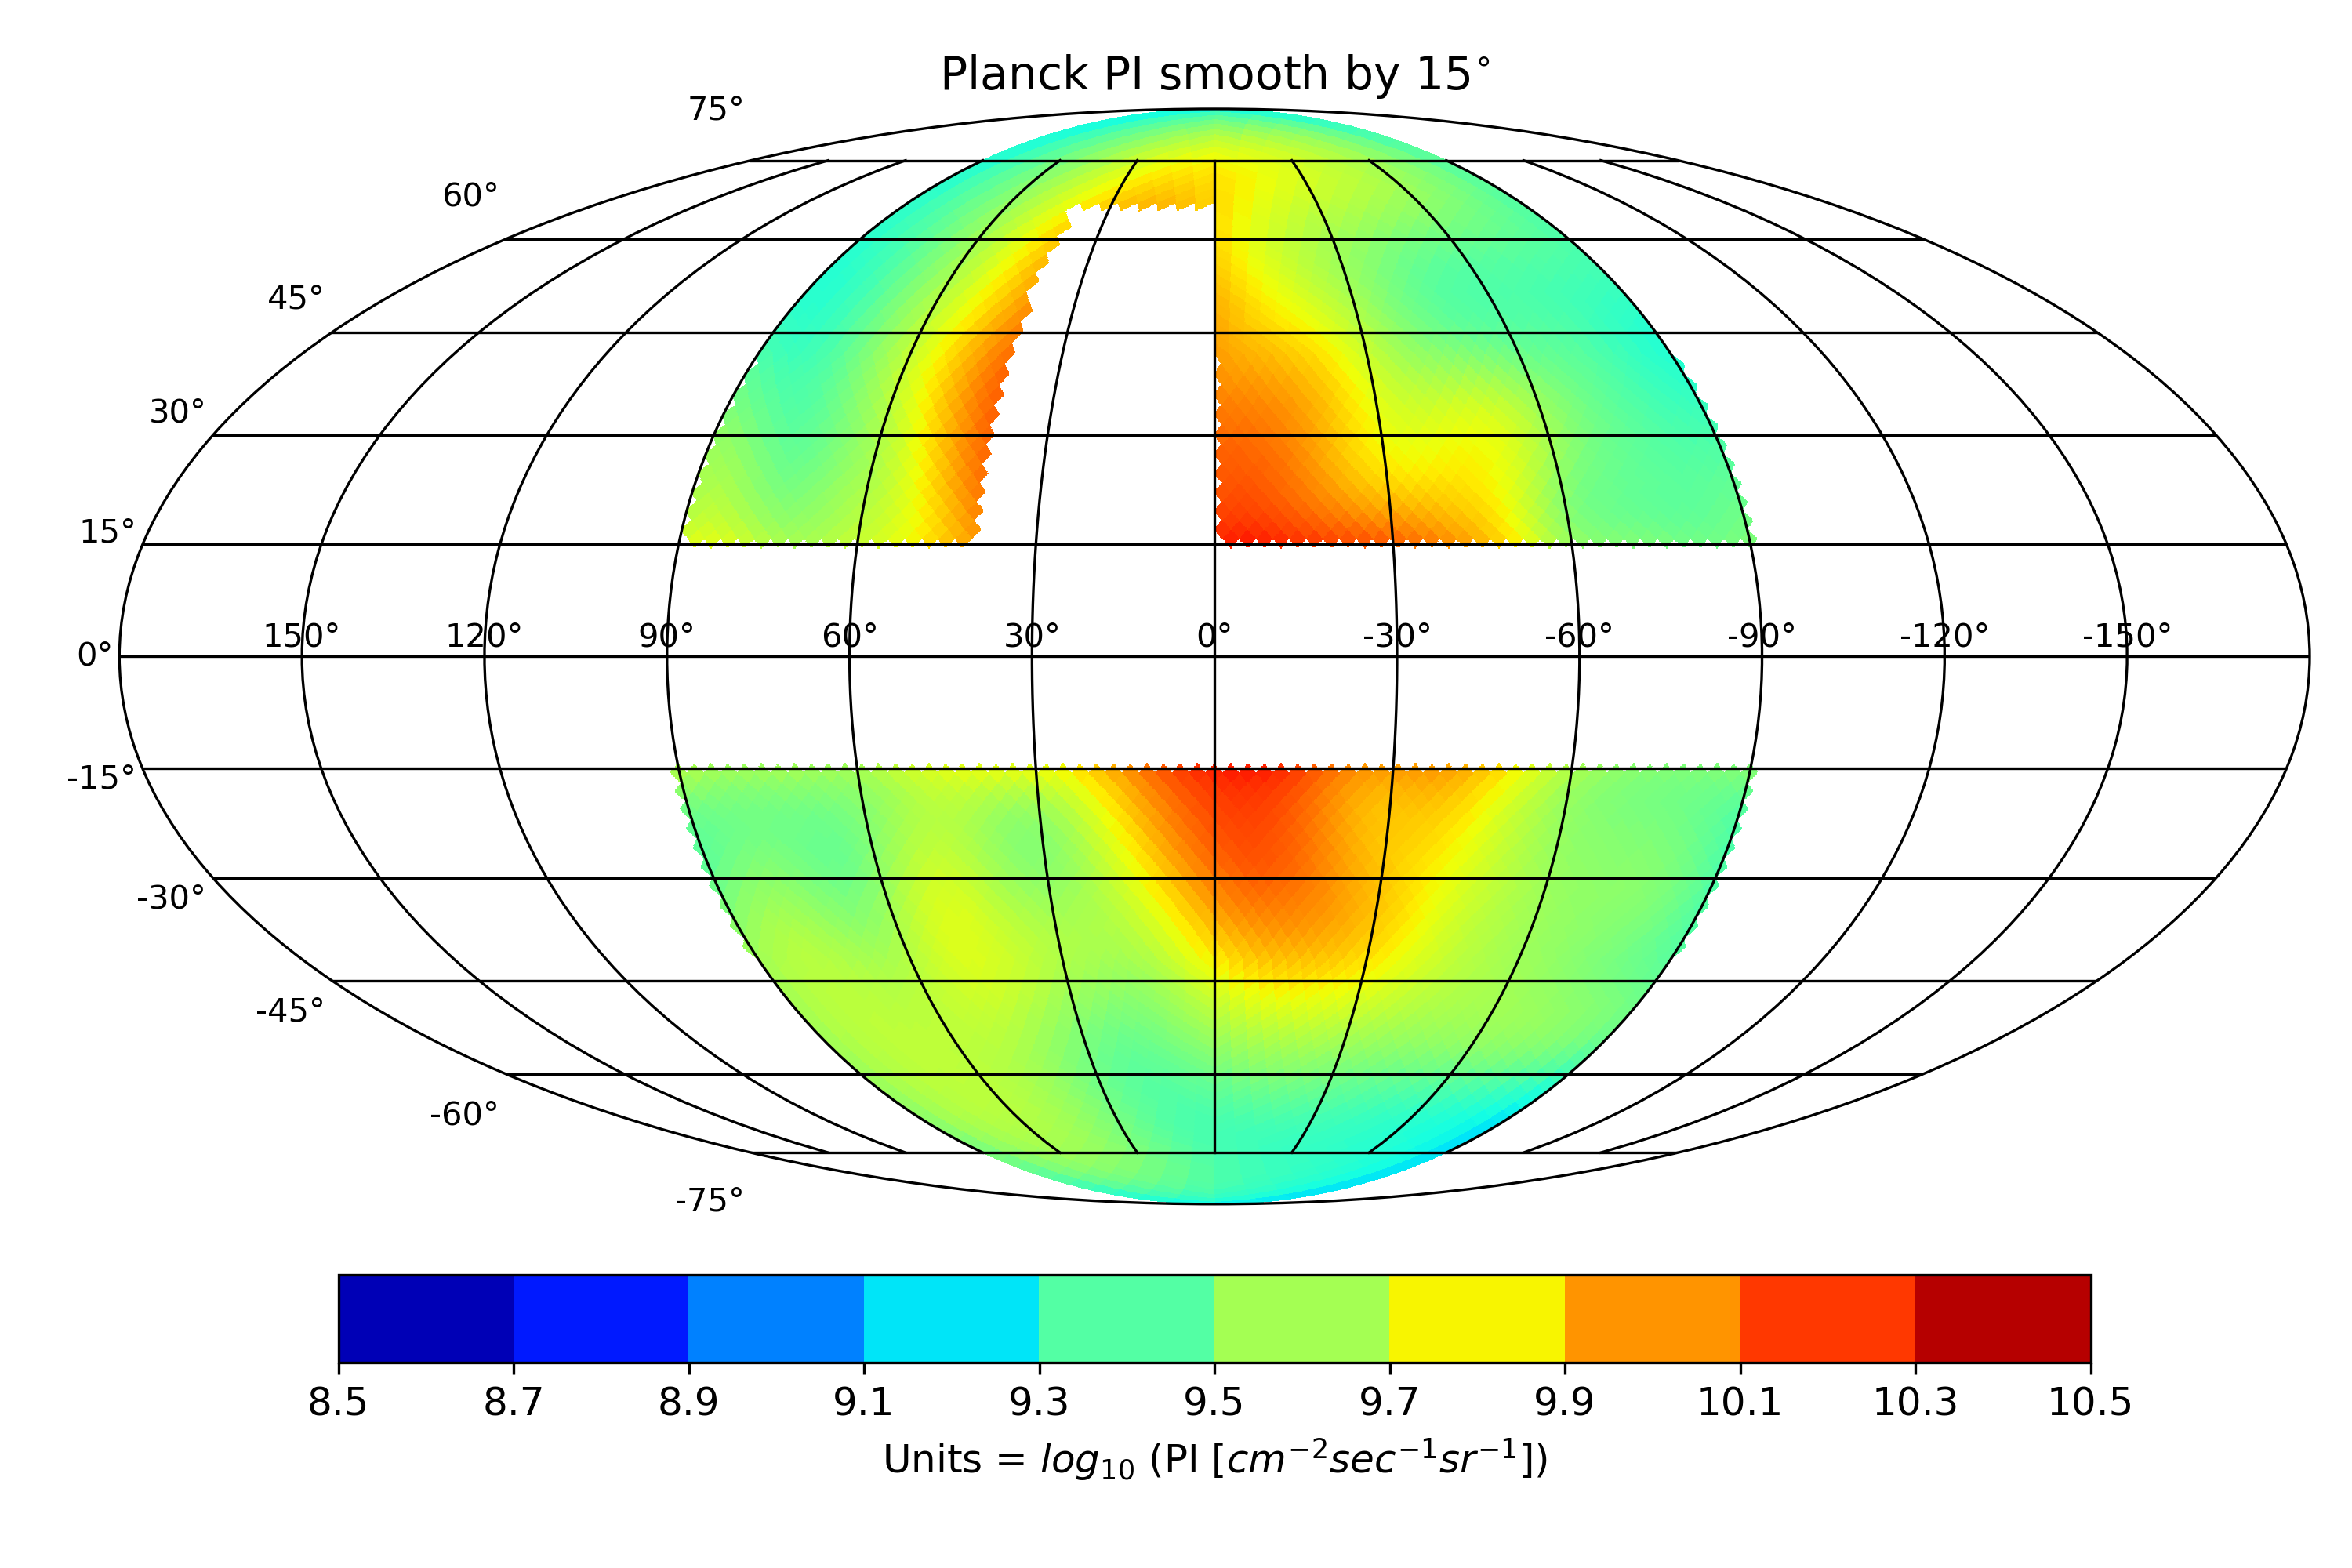
\includegraphics[width =9cm]{Images/Jan-08-2022_Planck_Sky_Map.png}%
        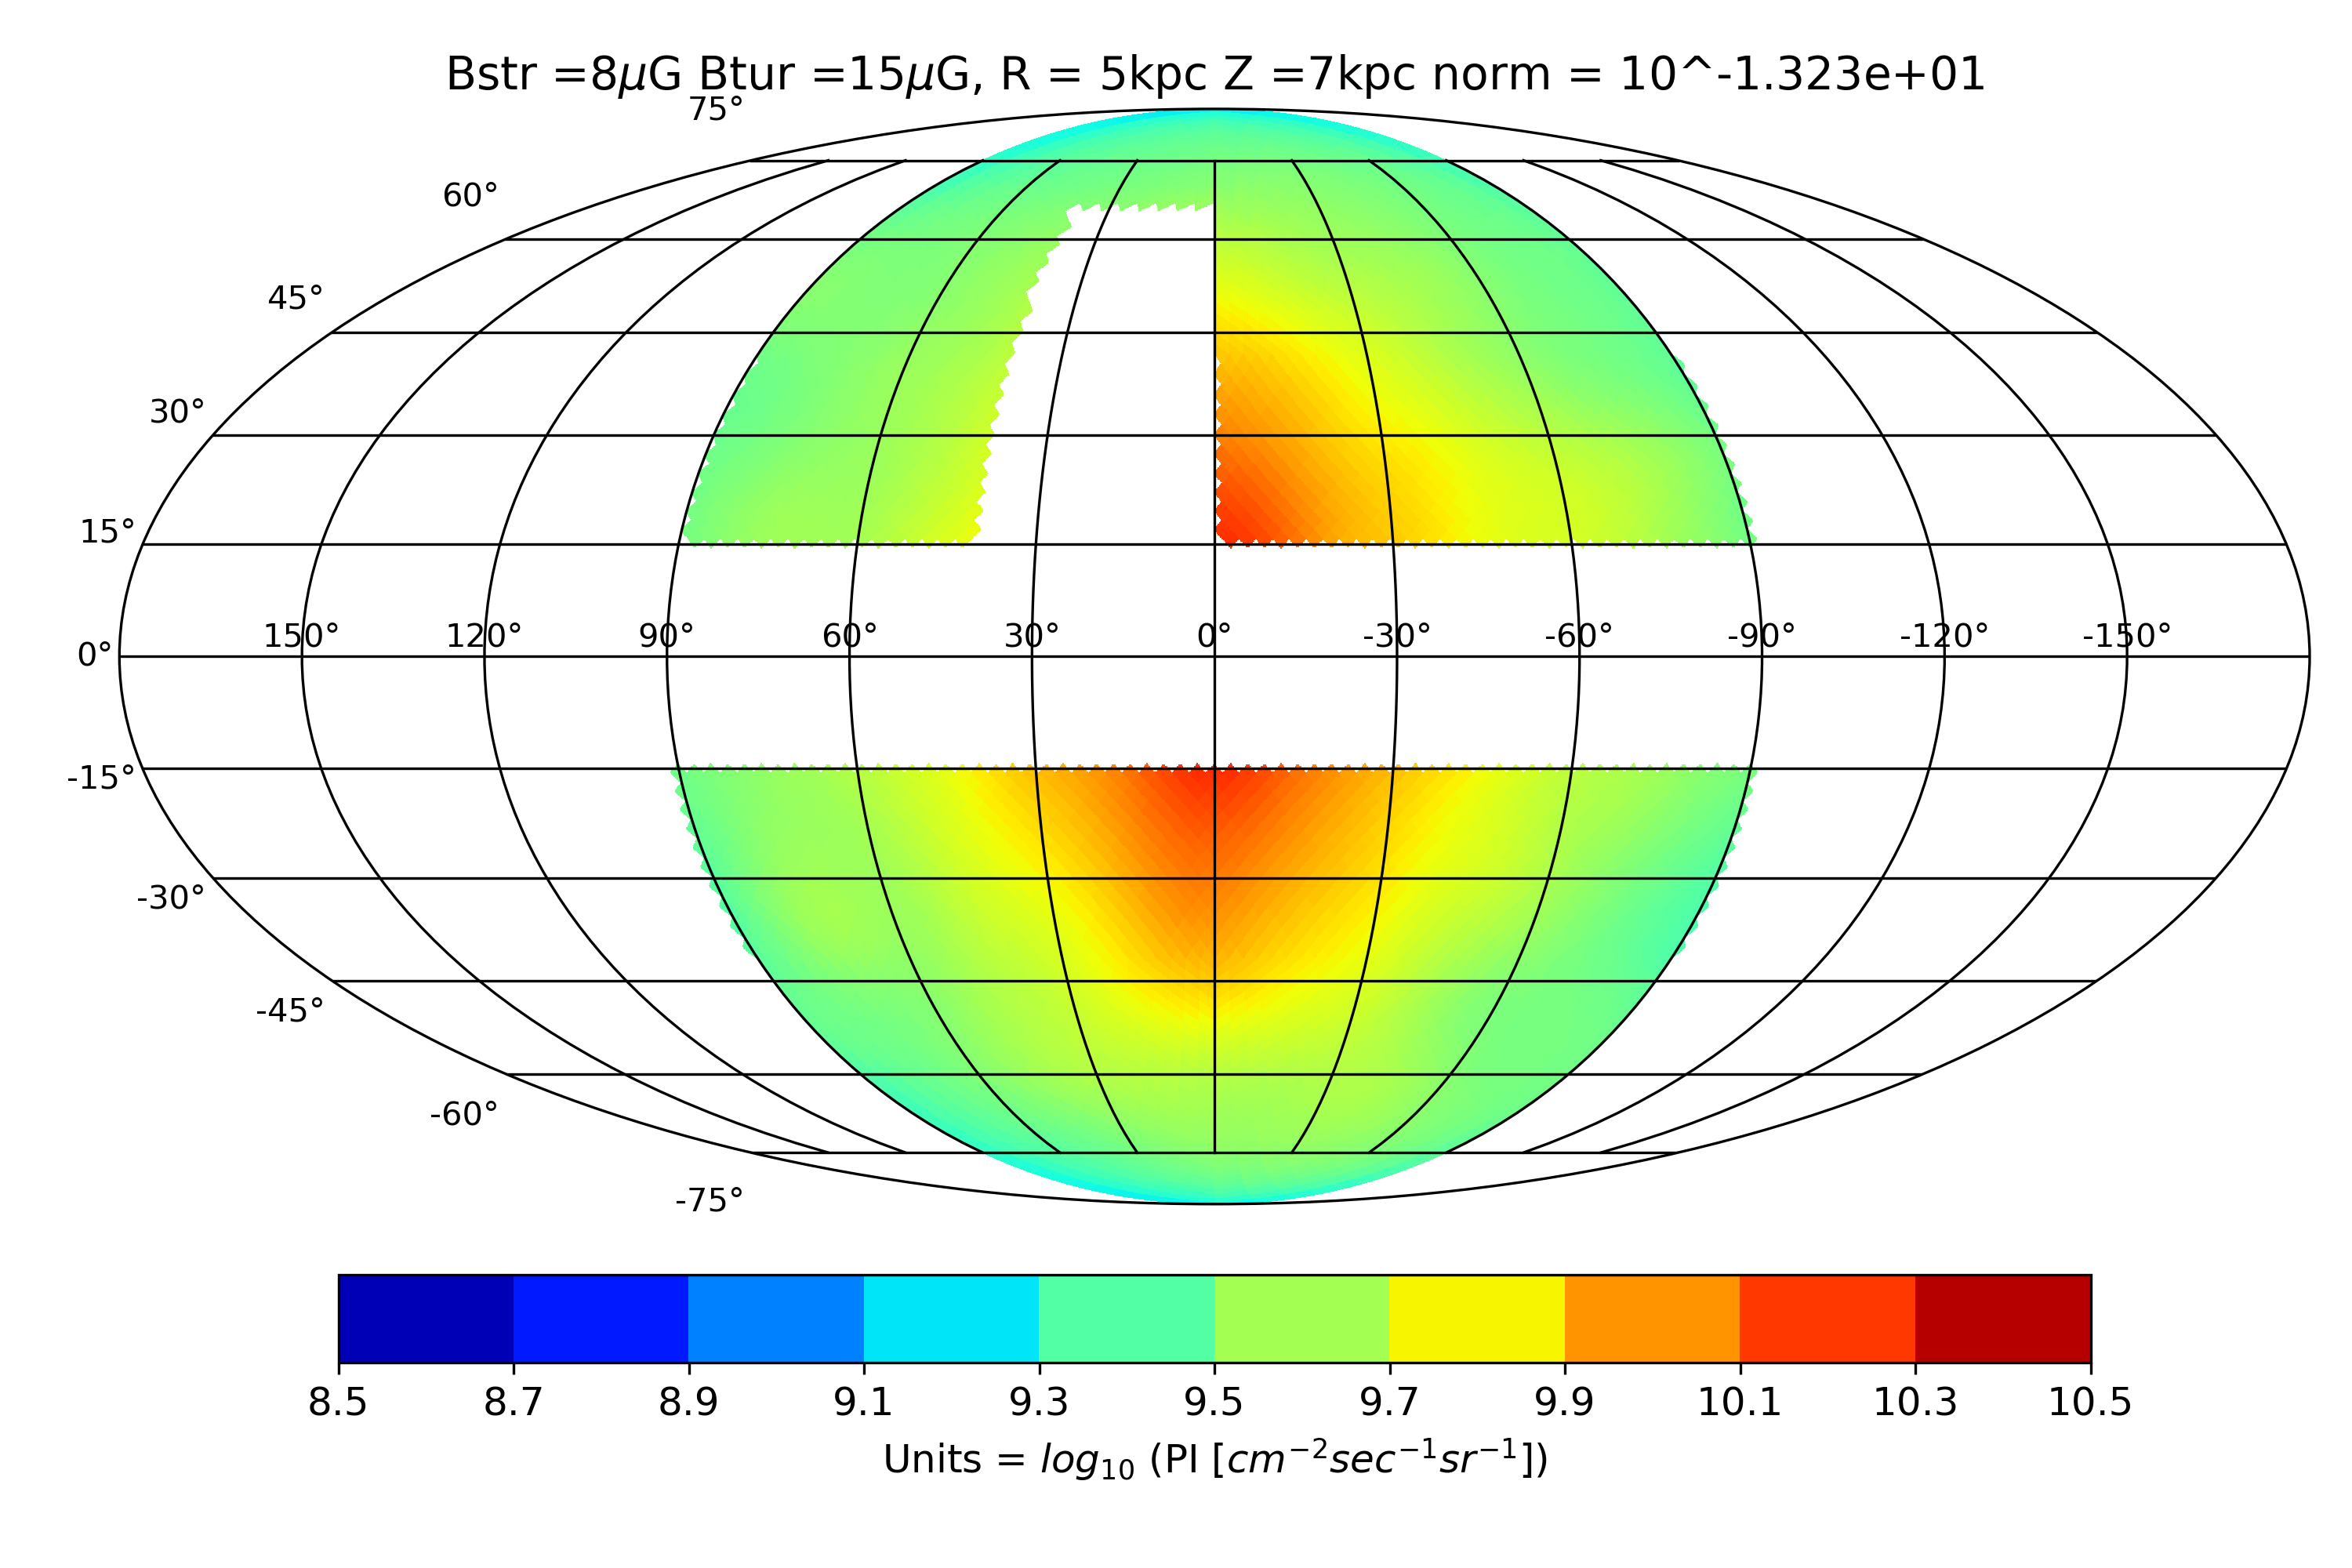
\includegraphics[width=9cm]{Images/Jan-08-2022_Skymap_Bstr_8_Btur_15_Rmag_5_Zmag_7_norm_-1.32e+01.png}
        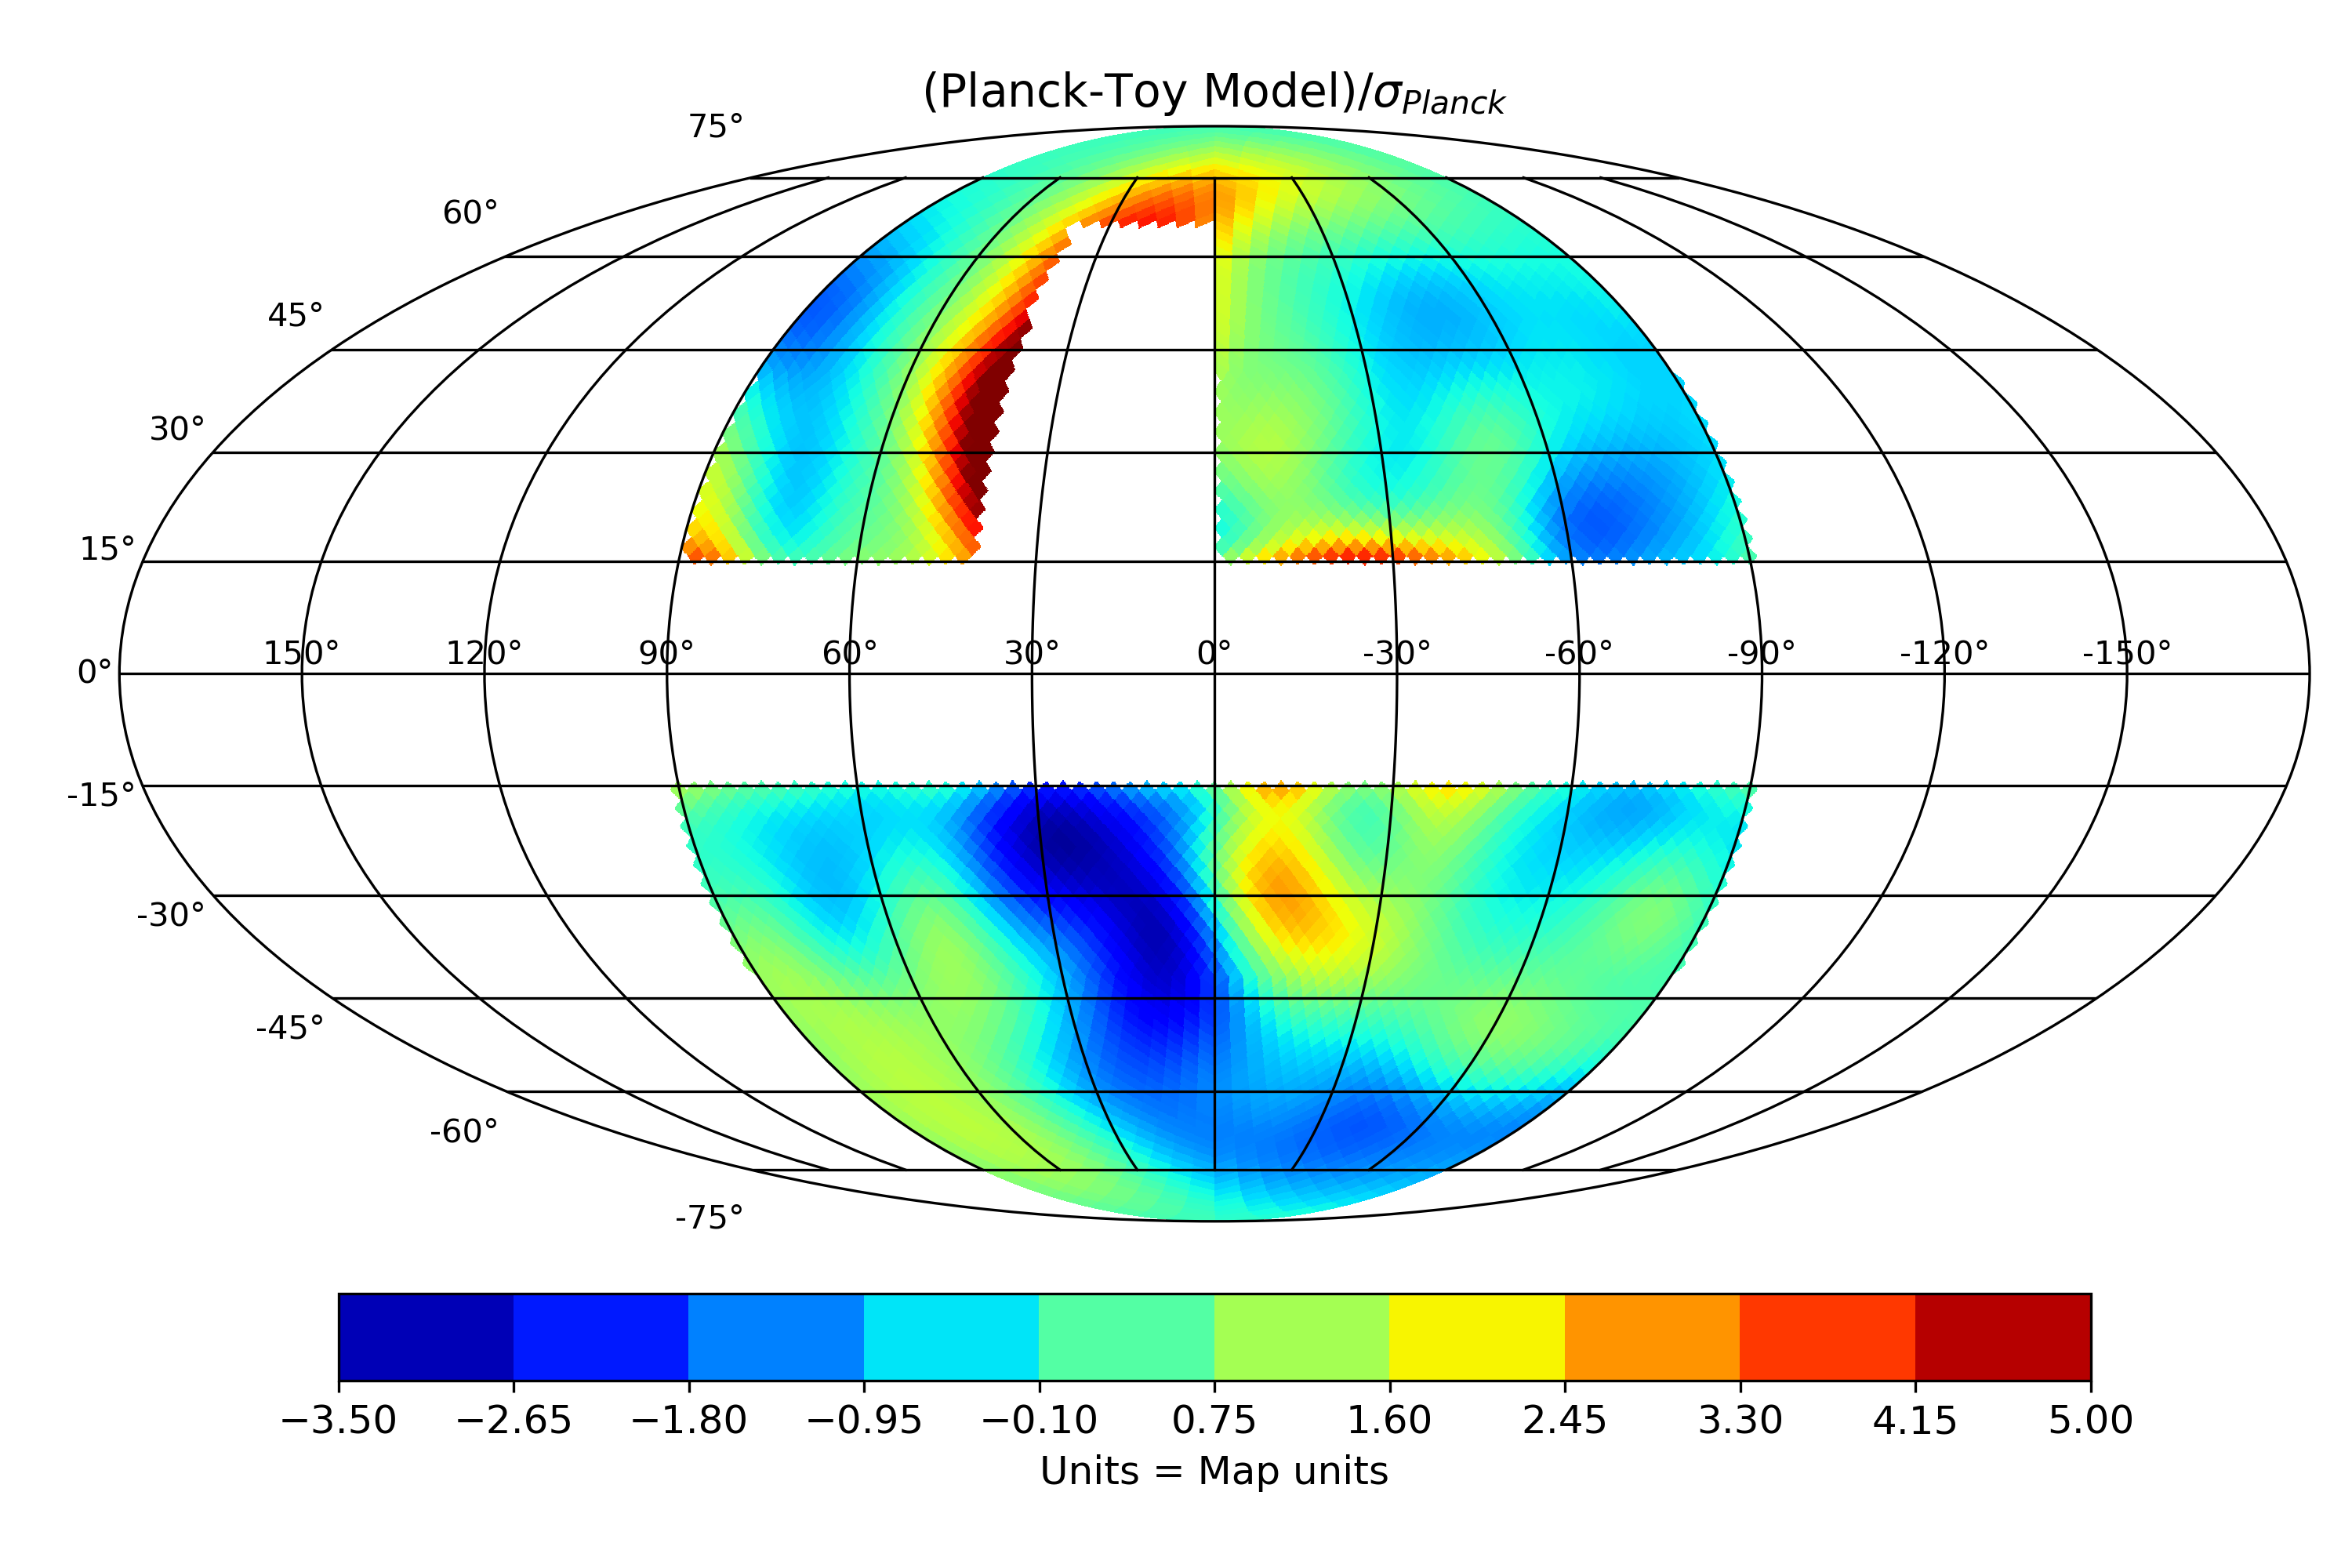
\includegraphics[width = 9cm]{Images/Jan-08-2022_Residue_Bstr_5_Btur_14_Rmag_5_Zmag_7_norm_-1.29e+01.png}
    \caption{Skymaps made for the latest value of minimum $\chi^2_{\rm dof} = 1.78$. Residuals for the same are below.}
    \label{fig:Skymaps}
\end{figure}
%% Polarisation fraction
We also estimate the polarisation fraction obtained by the toy-model which is given in figure \ref{fig:Pol_Frac} which was calculated taking the ratio of polarised intensity and total intensity. The polarisation fraction from the toy model is comparable to the values as seen in the observation data \cite{2013} and \cite{WMAP_Page}.


\begin{figure}[h!]
        \centering
        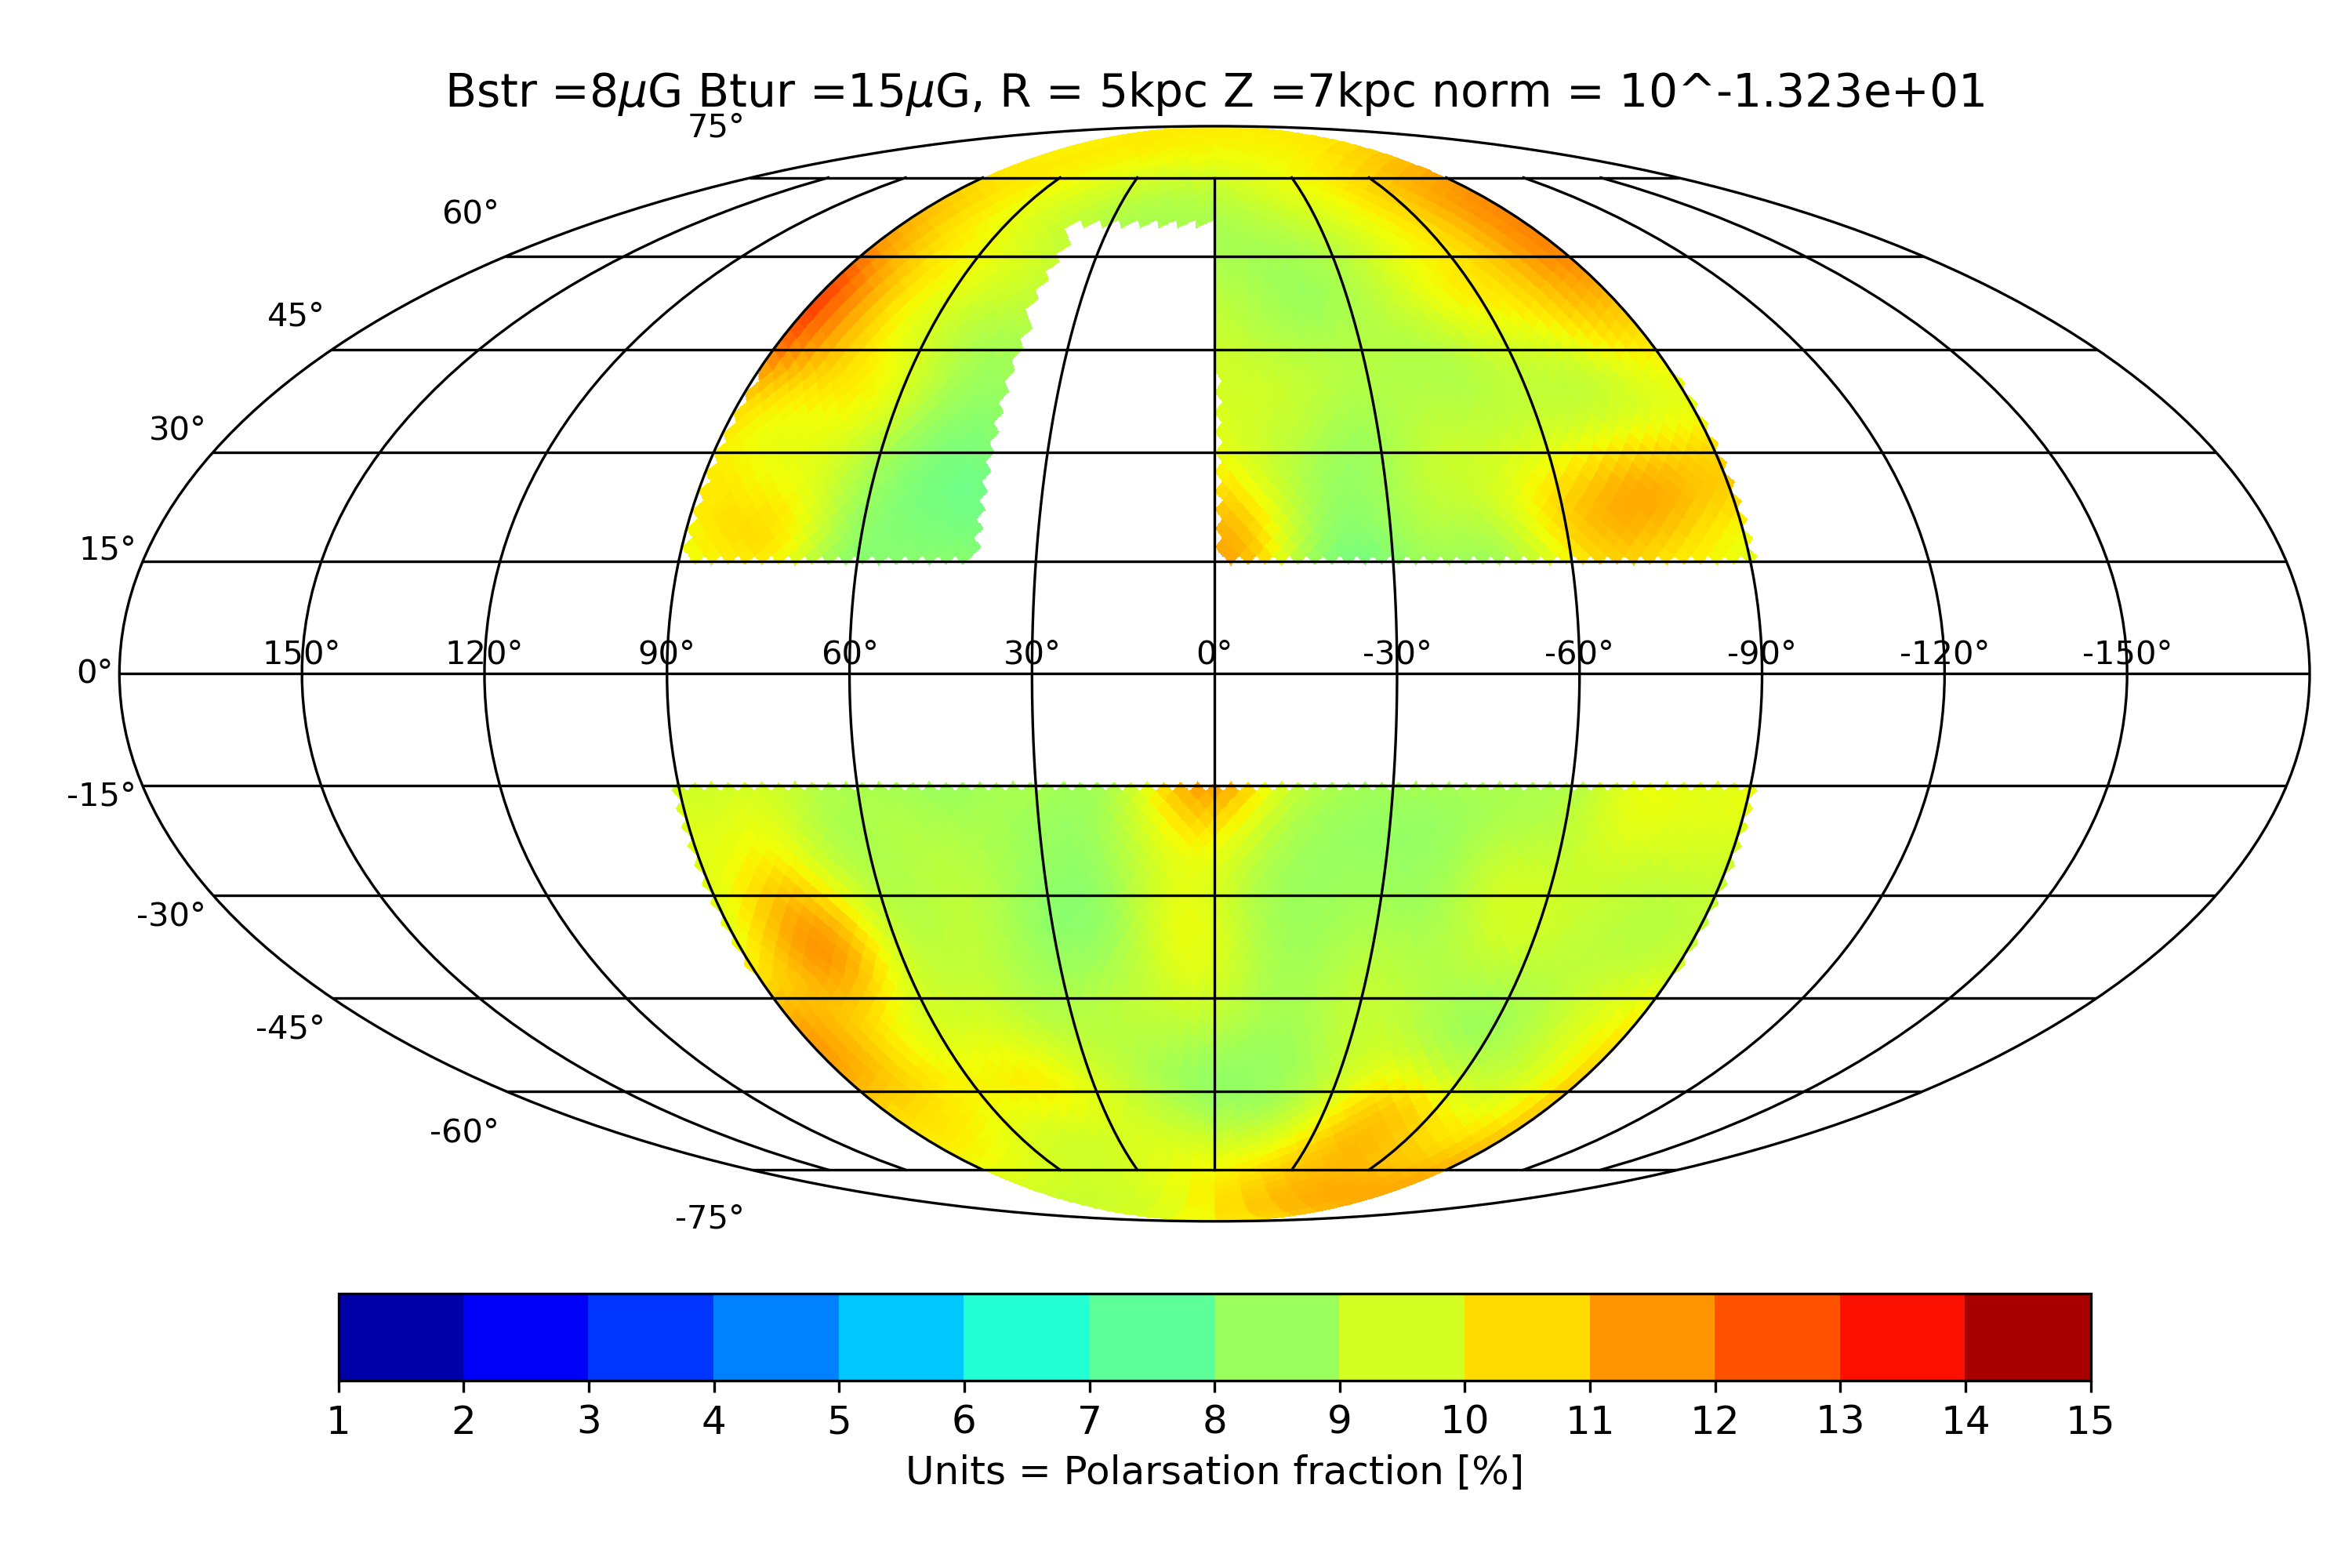
\includegraphics[width =9cm]{Images/Jan-09-2022Pol_Frac_30GHz_Total_Skymap_Bstr_8_Btur_15_Rmag_5_Zmag_7_norm_-1.32e+01.png}%
    \caption{Polarisation fraction obtained from the toy-model.}
    \label{fig:Pol_Frac}
\end{figure}

%% Uncertainities in the parameters
\label{Para_table}
%\setlength{\arrayrulewidth}{0.5mm}
%\setlength{\tabcolsep}{18pt}
%\renewcommand{\arraystretch}{1.5}
%\centering
\begin{center}
\begin{tabular}{ |p{2.cm}|p{4cm}|p{4cm}|  }
\hline
\multicolumn{3}{|c|}{Best-fit value with 1-$\sigma$ constraint} \\
\hline
Parameter & Best-fit value &Description \\
\hline
\hline
$B_{\mathrm{str}} $& $[8]^{2}_{9}$ ~ $\mu$G & Structured field strength \\
\hline
$B_{\mathrm{tur}} $& $ [15]^{4}_{} ~\mu$G & Turbulent field strength.\\
\hline
$R_{\mathrm{Mag}}$ = $R_{\mathrm{el}}$ & $[5]^{4}_{}$ ~kpc & Radial extent beyond which the field and electron distribution starts to drop. \\
\hline
$Z_{\mathrm{Mag}}$ = $Z_{\mathrm{el}}$ & $[7]^{6}_{}$~kpc & Height of the halo field for the toy model beyond which field starts to drop.\\
\hline
$C_{\rm norm}$ & $[10^{-13.230}]_{10^{-12.053}}$ ${\rm cm}^{-3}$ & Normalisation factor for the electron distribution.\\
\hline
\end{tabular}
\end{center}

In table ~\ref{Para_table} we provide the list of all free parameters and the constraints obtained on them. The spatial parameters $R_{\mathrm{Mag}}$ = $R_{\mathrm{el}}$ and $Z_{\mathrm{Mag}}$ = $Z_{\mathrm{el}}$ for magnetic field and electron distribution extent has been kept the same. The reason for this constrain is that synchrotron radiation will only be emitted when both non-thermal electrons and magnetic fields are present. Hence even if the geometry of the fields differ from the electron distribution we can only probe it in the regime where both fields and electrons are present.
\newline
%We obtained $1\sigma$ constraint for $B_{\mathrm Mag}$ = [2,9]$\mu$ G,$B_{\mathrm tur}$ = [4,15)$\mu$ G , $R_{\mathrm Mag}$ = [4,5), $Z_{\mathrm Mag}$ = [6,7) and $C_{\mathrm norm}$= $\mathrm{(5\times 10^{-14},8.83}\times 10^{-13}]$. 

\begin{figure}[h!]
        \centering
        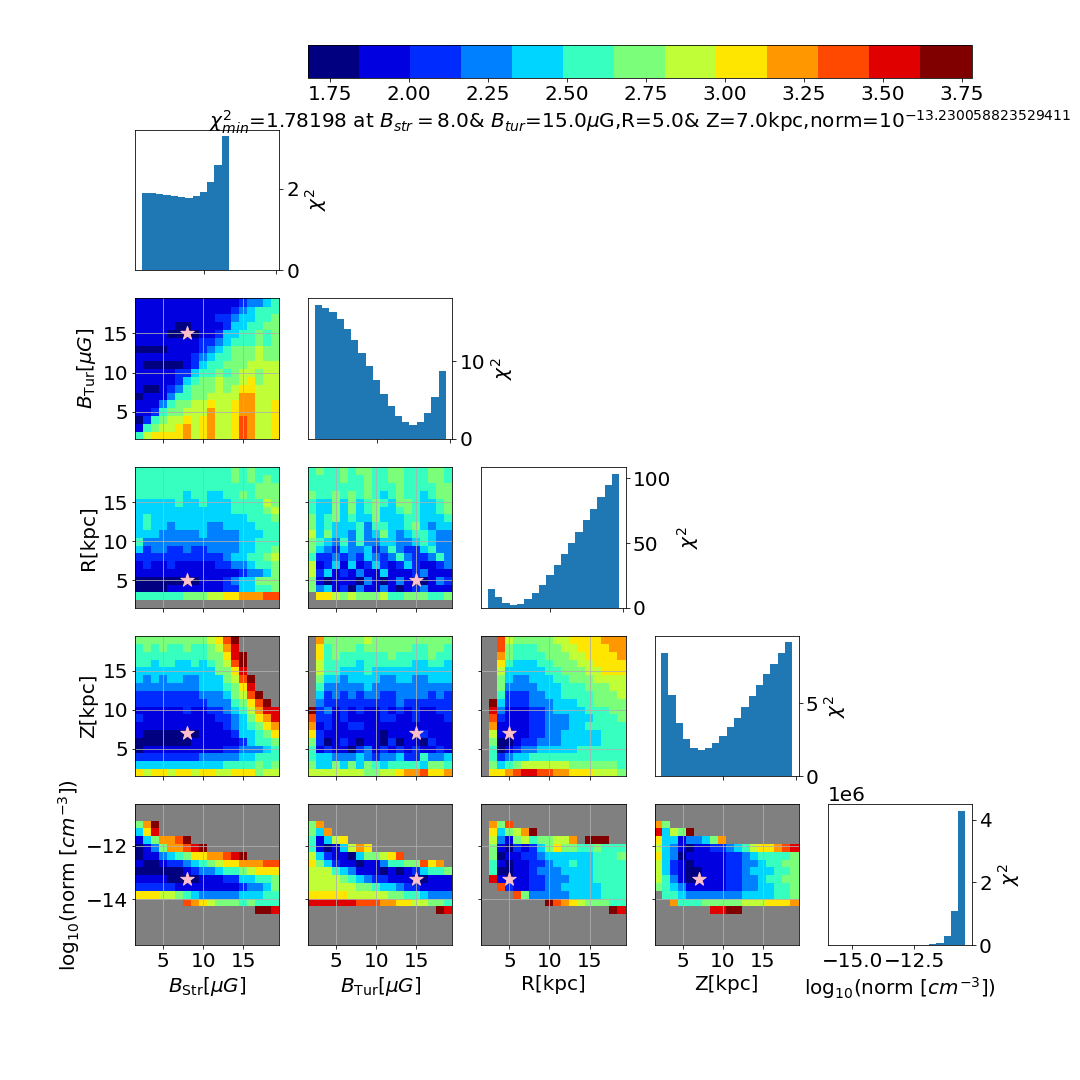
\includegraphics[width = 10cm]{Images/Jan8_Chsq_dof_Para_Scan_1_9_3_elec_den_norm_10GeV.png}
        \caption{\Vasu{1 million value parameter scan}}
        \label{fig:my_label}
\end{figure}




\begin{itemize}
 
    \item Arrival directions from cosmic rays-comparison between JF12 halo fields and toy model halo fields at 100 EeV and 30 EeV for protons and nitrogen.
    \item Uncertainities in parameter values propagate large errors in arrival direction of cosmic rays.
\end{itemize}
\newpage
\subsection{Jan 8-Comparison with Planck data and Parameter Estimation}





\subsection{Cosmic ray deflections from different magnetic field models}

The effect of Galactic halo fields on the arrival directions of UHECRs was the other focus of our study. We use JF12 model as a comparison for our toy model. The JF12 model has very weak fields both in the structured and turbulent fields in the halo. Our parameter scan results provide a very poor constraints on the parameters and this implies that we will propagate a lot of uncertainties in our arrival direction calculation. Hence, we use the equipartition constraint which provided a stronger bounds on the parameters as shown in figure[\ref{Equipartition}]. We use two combinations of parameters one where we obtain the smallest values and the other where we have the largest values.

\begin{figure}[h!]
    \centering
    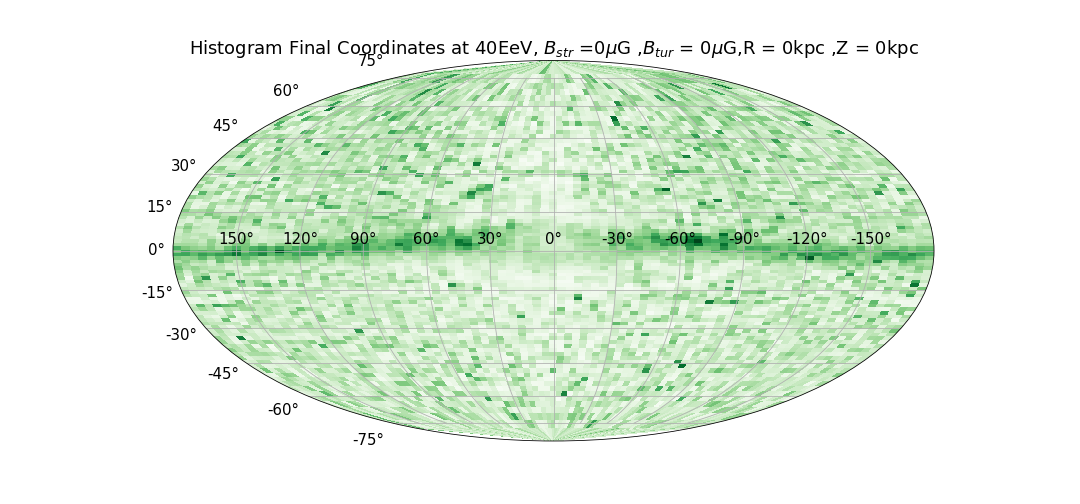
\includegraphics[width = 14cm]{Images/JF12_Proton_Final_Coordinates_Hist_Energy40_Bstr_0_Btur_0_R_0_Z_0.png}%
    \caption{\rm {JF12 Toroidal halo} Histogram from backtracking of cosmic ray protons. 90 bins in latitude and longitude.}
    \label{fig:my_label}
\end{figure}


\newgeometry{top=20mm, bottom=20mm,lmargin=1.mm,rmargin=1.mm}   
\subsection{Arrival directions from CenA and NGC253 for JF12 and toy model}

\begin{figure}[h!]
    \centering
    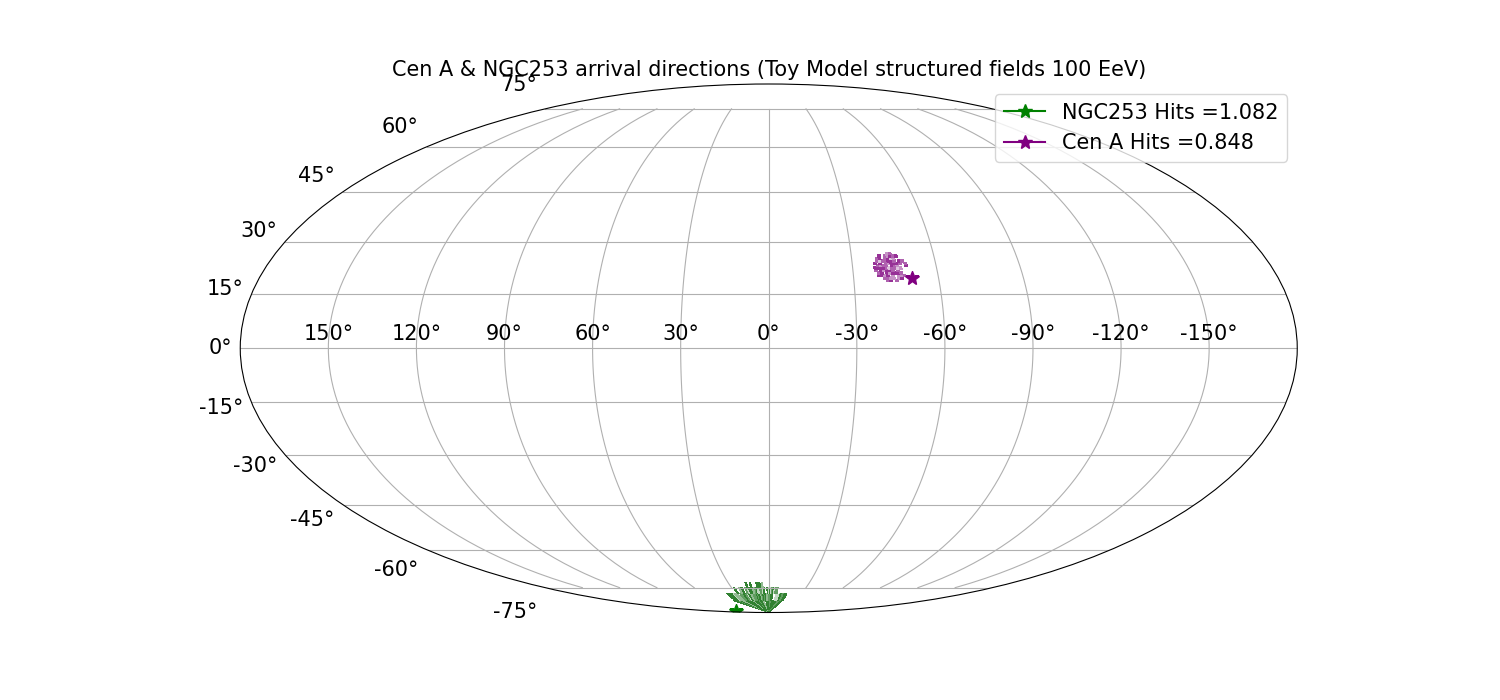
\includegraphics[width = 10cm]{Images/CenA_NGC253_Str_TM_100EeV.png}%
    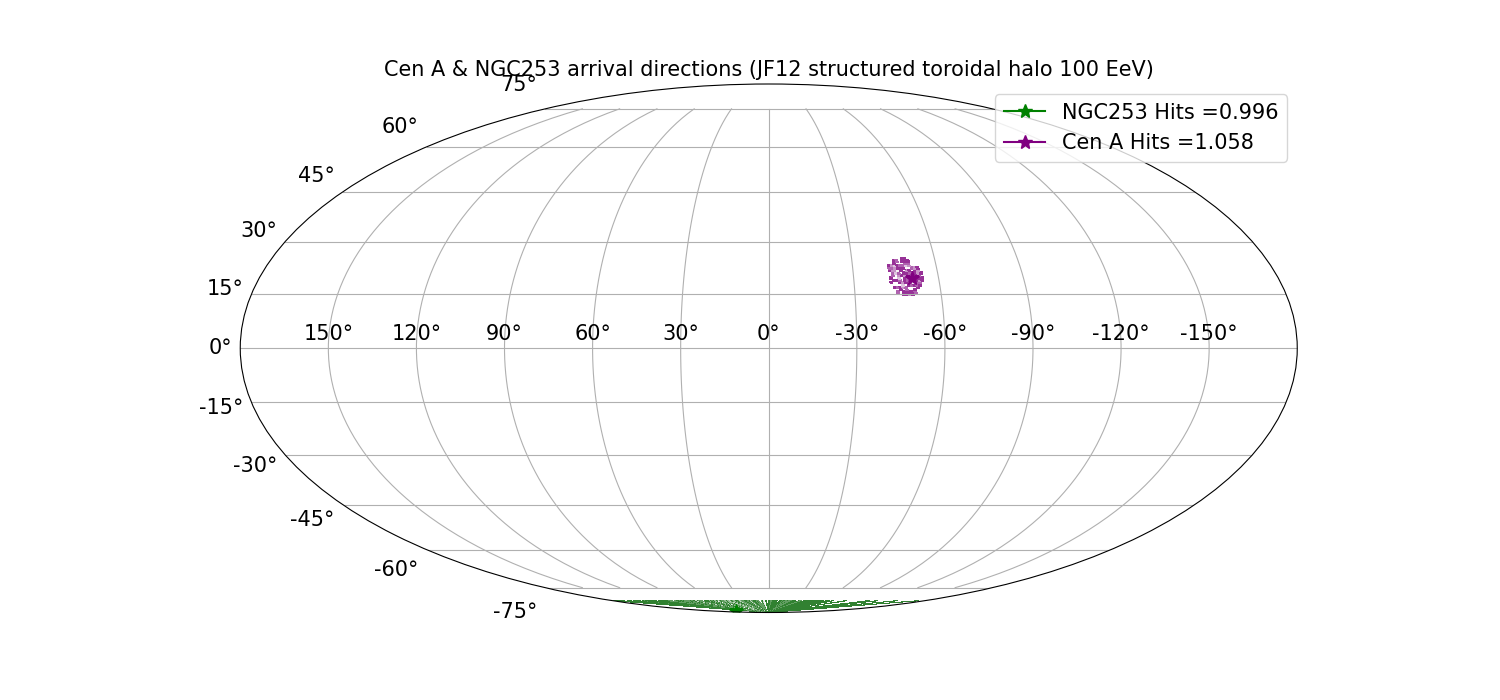
\includegraphics[width = 10cm]{Images/CenA_NGC253_Str_JF12_100EeV.png}
    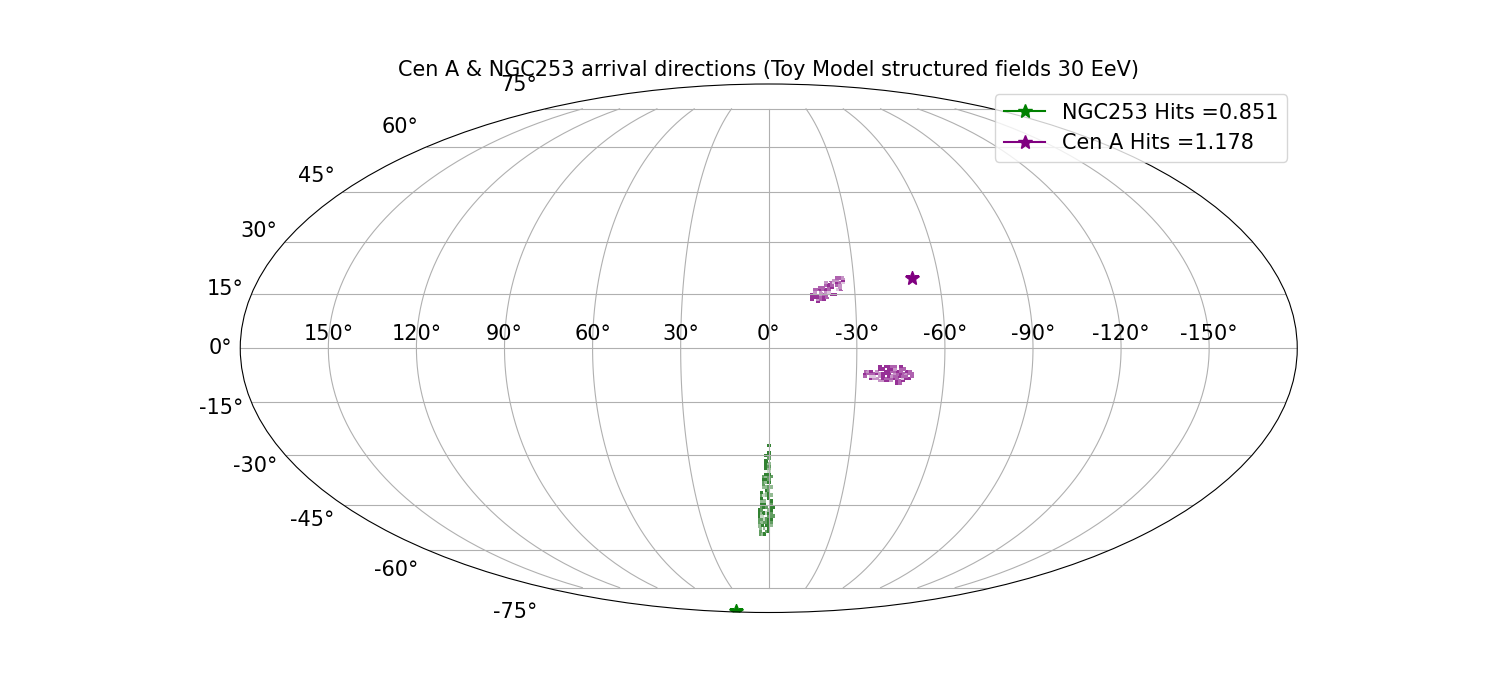
\includegraphics[width = 10cm]{Images/CenA_NGC253_Str_TM_30EeV.png}%
    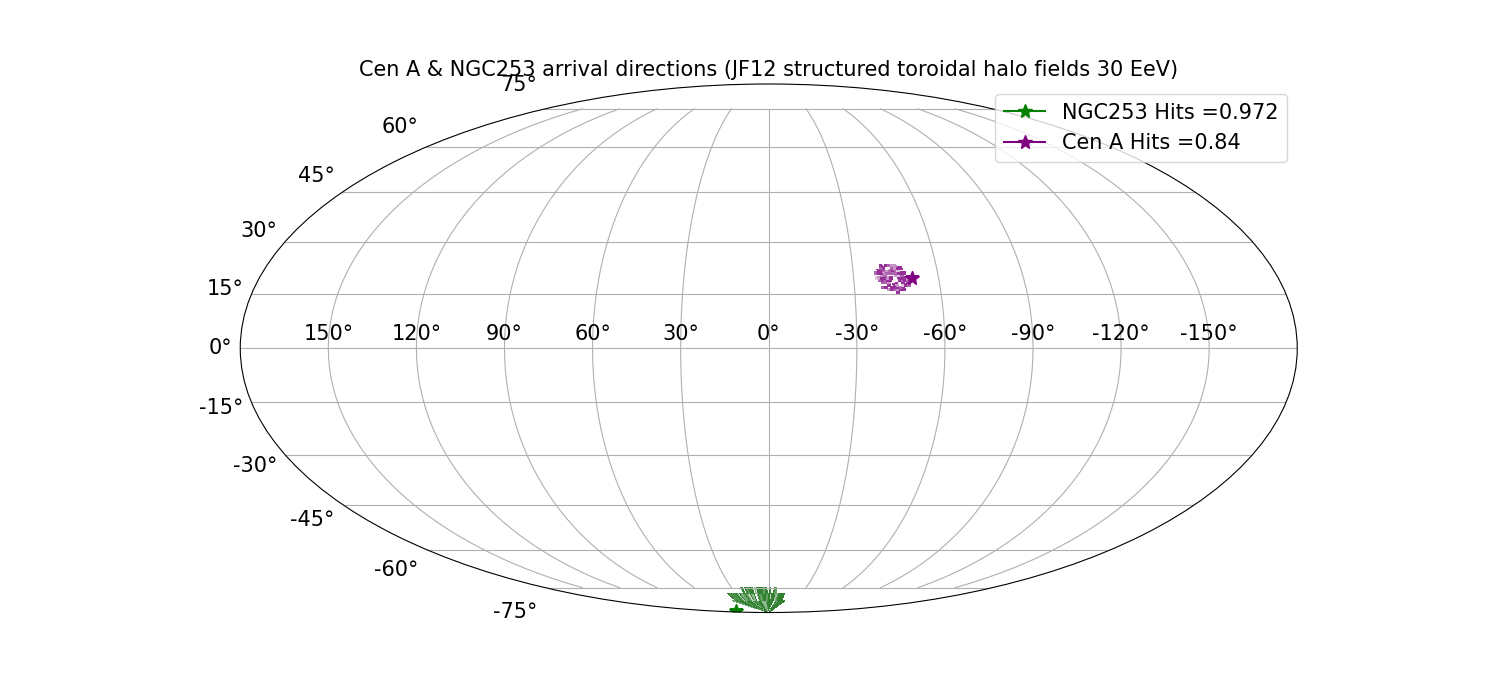
\includegraphics[width = 10cm]{Images/CenA_NGC253_Str_JF12_30EeV.png}
    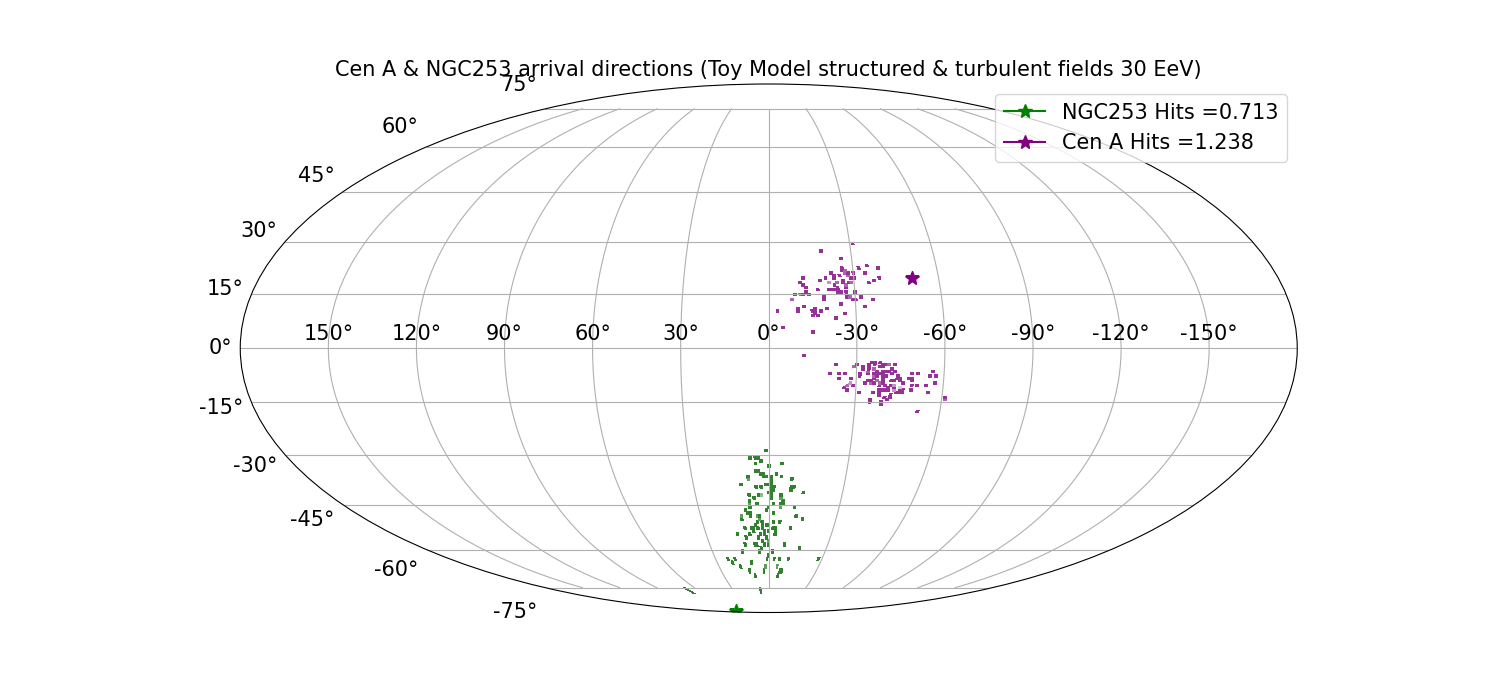
\includegraphics[width =10cm]{Images/CenA_NGC253_Str_Tur_TM_30EeV.png}%
    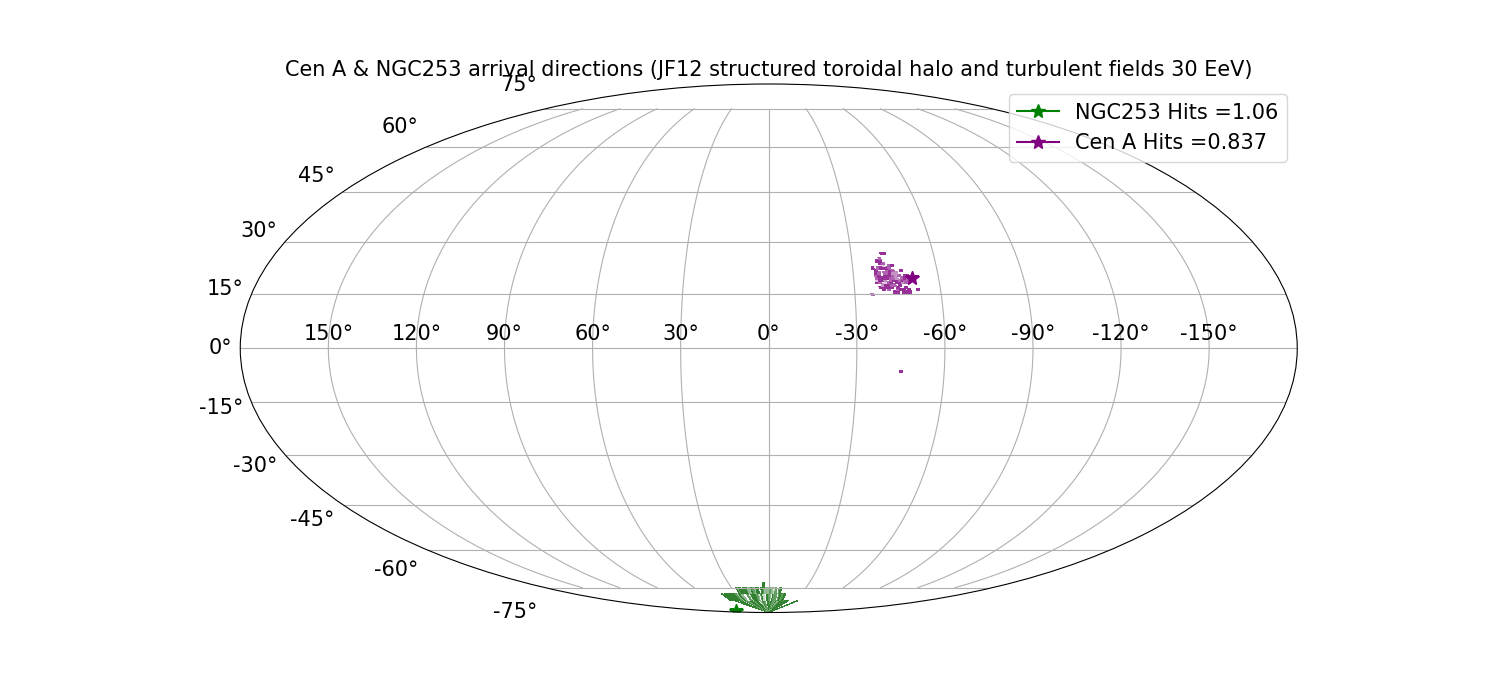
\includegraphics[width = 10cm]{Images/CenA_NGC253_Str_Tur_JF12_30EeV.png}
    \caption{Arrival directions for CenA and NGC253 for $B_{str} = 6\mu$G,$B_{tur} =10\mu$G ,$R = 12kpc$ and $Z = 7$kpc.}
    \label{fig:my_label}
\end{figure}
\restoregeometry

\newpage
\newgeometry{top=20mm, bottom=20mm,lmargin=1.mm,rmargin=1.mm}   
\subsection{Arrival directions from sources on a Grid}
\begin{figure}[h!]
    \centering
    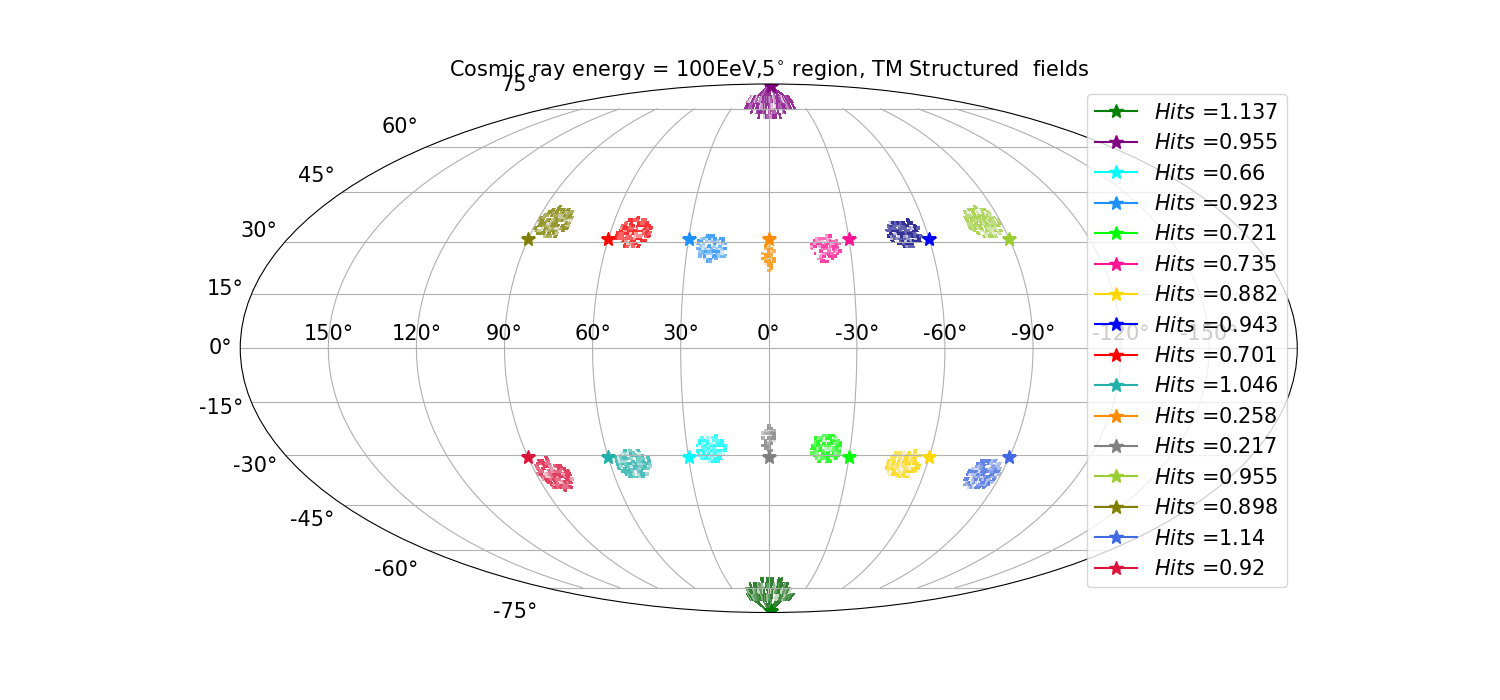
\includegraphics[width = 10cm]{Images/Str_TM_particles1e5_100EeV (1).png}%
    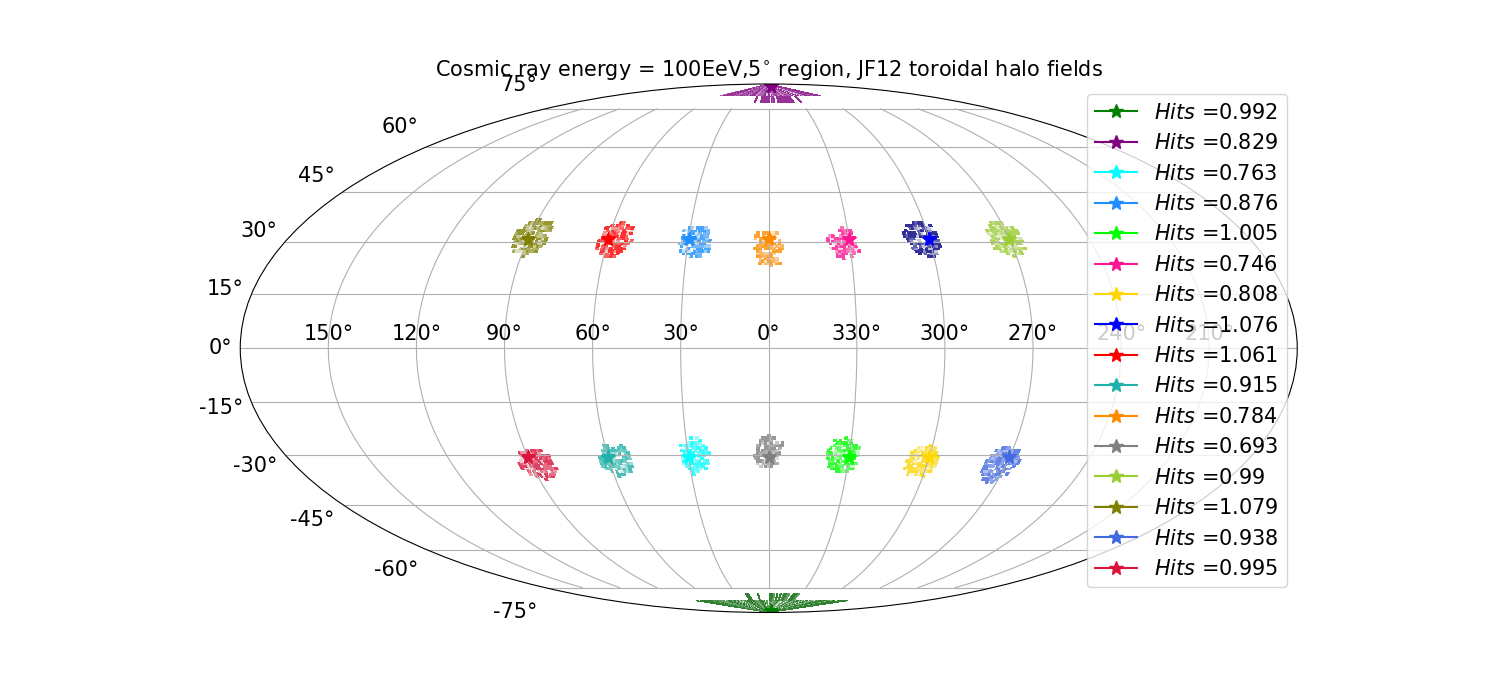
\includegraphics[width=10cm]{Images/JF12_TorH_particles1e5_100EeV (1).png}
    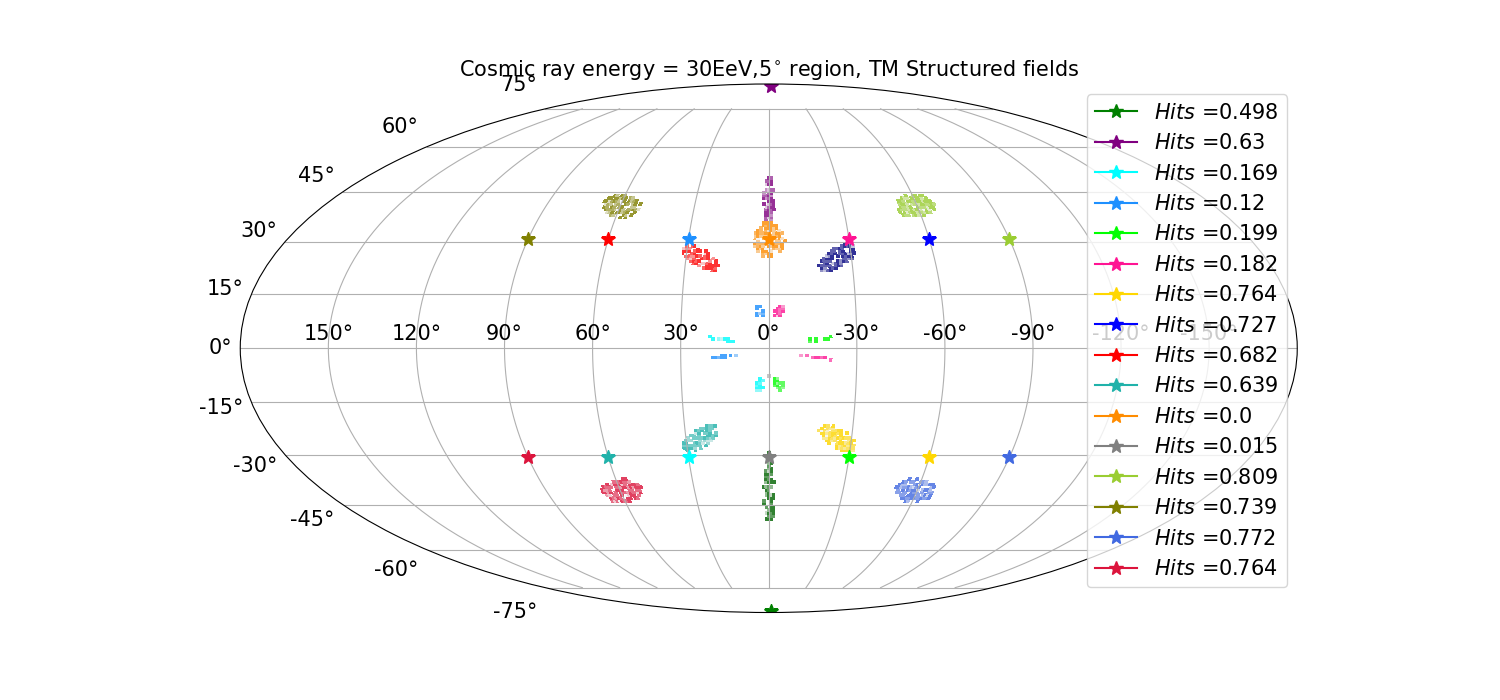
\includegraphics[width = 10cm]{Images/Str_TM_particles1e5_30EeV (1).png}%
    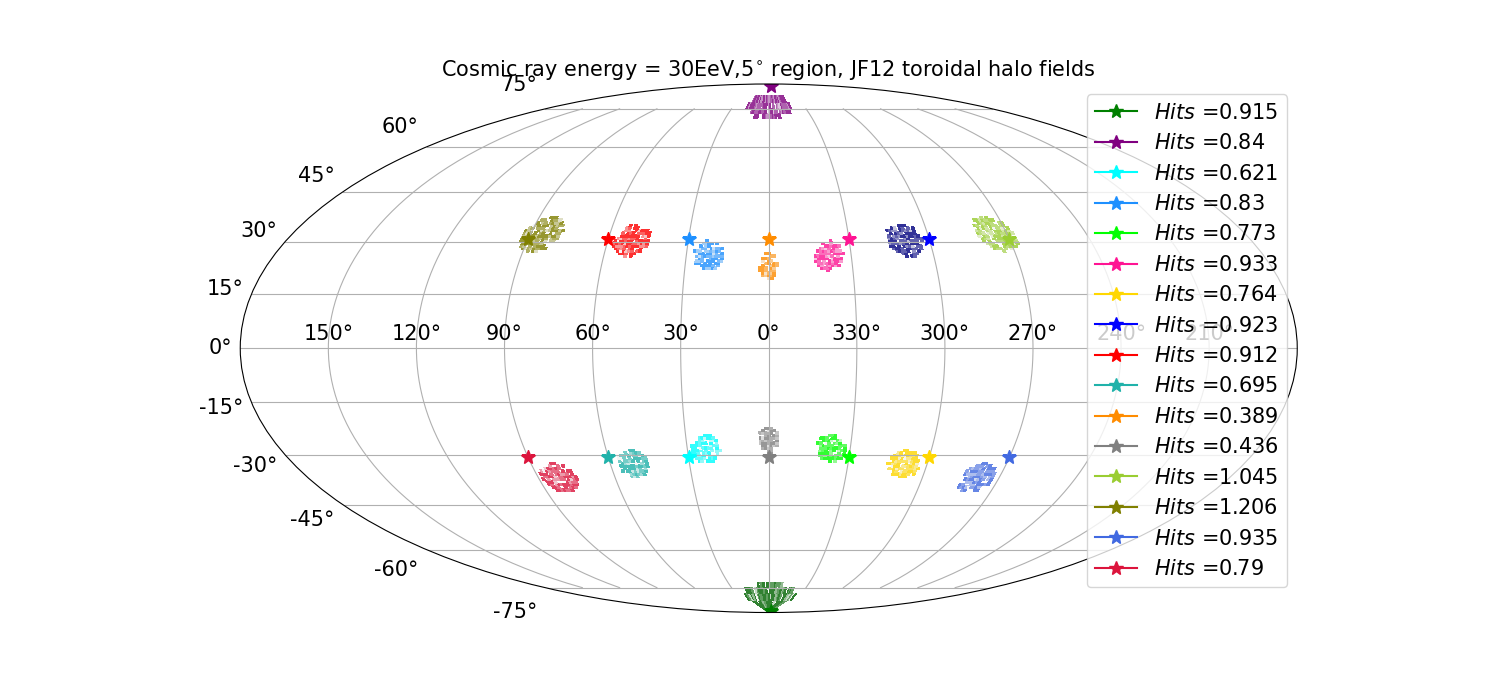
\includegraphics[width = 10cm]{Images/JF12_TorH_particles1e5_30EeV (1).png}
    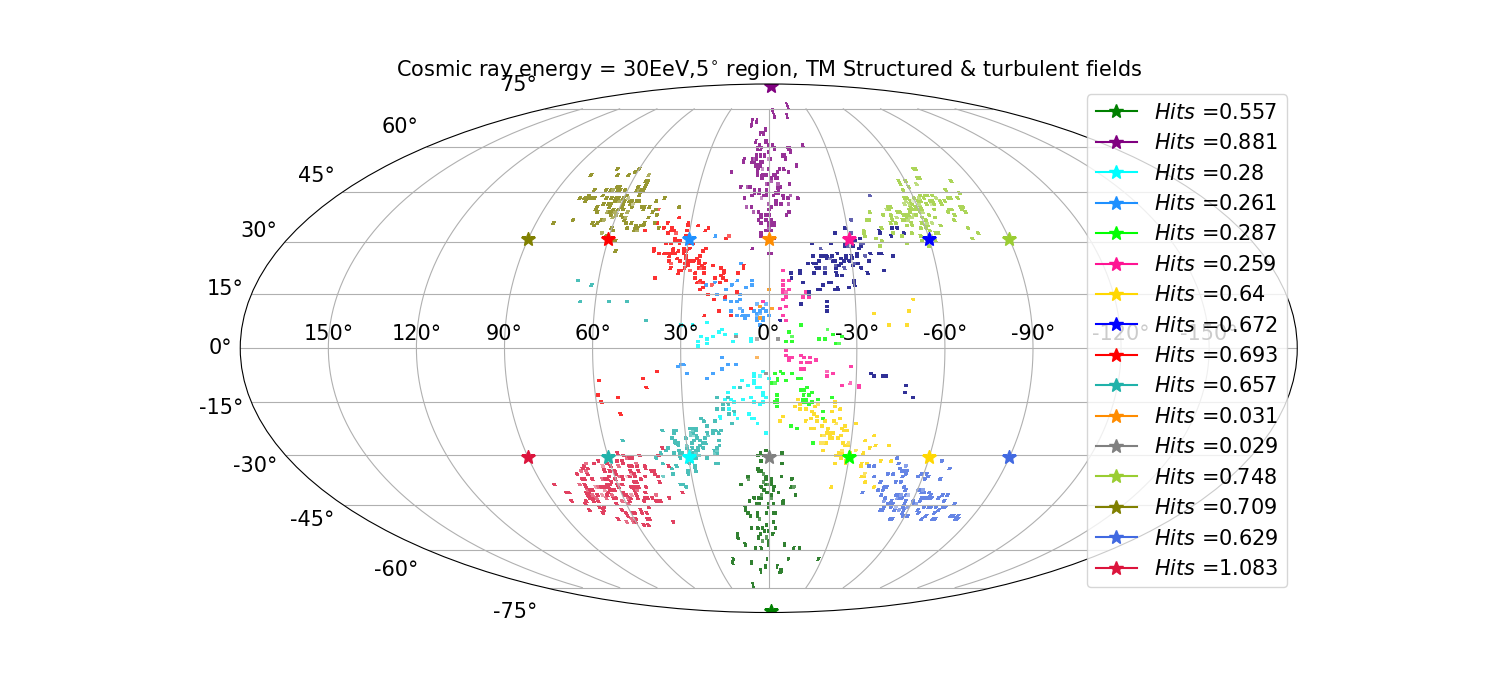
\includegraphics[width = 10cm]{Images/Tur_Str_TM_particles1e5_30EeV (1).png}%
    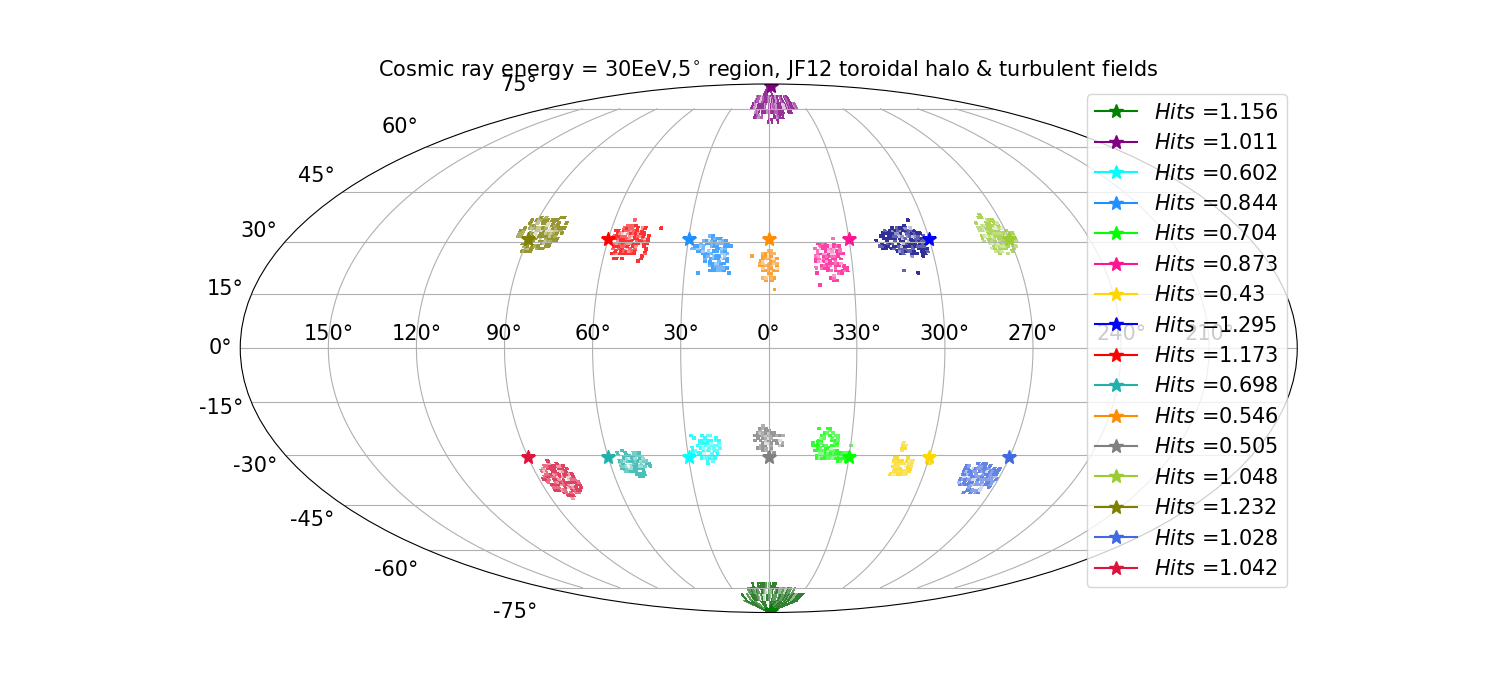
\includegraphics[width = 10cm]{Images/JF12_TorH_Tur_particles1e5_30EeV (1).png}
    \caption{Arrival directions for sources on a Grid for $B_{str} = 6\mu$G,$B_{tur} =10\mu$G ,$R = 12kpc$ and $Z = 7$kpc.}
    \label{fig:my_label}
\end{figure}
\restoregeometry
\section{Conclusions}
\clearpage
\section{References}

\printbibliography[heading=none]

\nocite{*}

\newpage
\section{Appendix A}\label{Appendix_A}
As discussed in section(\ref{Synchrotron_theory}) the line of sight components for Stokes parameters is given by:
\begin{eqnarray}
Q^l_{\rm in} = ({J_{\perp}^l} - J_{\parallel}^l) \ {\cos}(2\Psi^l_{\rm in}) \ \\ U^l_{\rm in} = ({J_{\perp}^l} - J_{\parallel}^l) \ {\sin}(2\Psi^l_{\rm in}) \ .
\end{eqnarray}
We can take two test cases (I \& II) given in figure(\ref{fig_tot_intensity}) and figure (\ref{fig_pol_intensity}) respectively.We consider that there are two steps along a line of sight for which ${J_{\perp}^{(1,2)}}$ = 0.85 and $J_{\parallel}^{(1,2)}$  = 0.15. 
\\ In case I the angles $\Psi_{\rm in}^{(1,2)}$ = $90^{\circ}$ \& $0^{\circ}$. The resultant value of $I_{\rm pol}$ = 0 by virtue of eq.(\ref{eq_I_pol}) and we only have a contribution in $I_{\rm tot}$. This implies that for case I the resultant emission is seen only in total intensity since the values of $J_{\perp}^{\rm tot}$ = $J_{\parallel}^{\rm tot}$. 
\\ In case II we apply similar calculations to case I however, now the angles are $\Psi_{\rm in}^{(1,2)}$ = $90^{\circ}$ \& $45^{\circ}$. This in turn results in contribution to both polarised emission $I_{\rm pol}$ and total intensity $I_{\rm tot}$. Thus the values of $J_{\perp}^{\rm tot} \neq J_{\parallel}^{\rm tot}$. In figure(\ref{fig_pol_intensity}) we only show polarised intensity for simplicity however, there will be both total intensity and polarised intensity present.
\begin{figure}[h!]
     \centering
     \begin{subfigure}{0.4\textwidth}
         \centering
         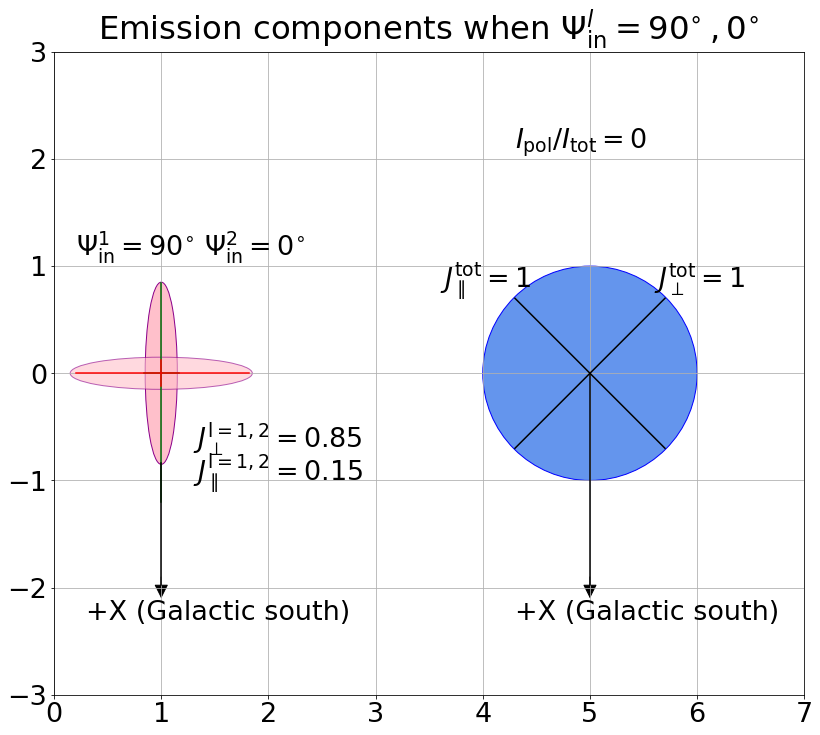
\includegraphics[width = 7cm]{Images/Total_intensity_Ellipses_circles_emissions.png}
         \caption{Case I - Total intensity}
         \label{fig_tot_intensity}
     \end{subfigure}
  \hfill
    \begin{subfigure}{0.4\textwidth}
         \centering
         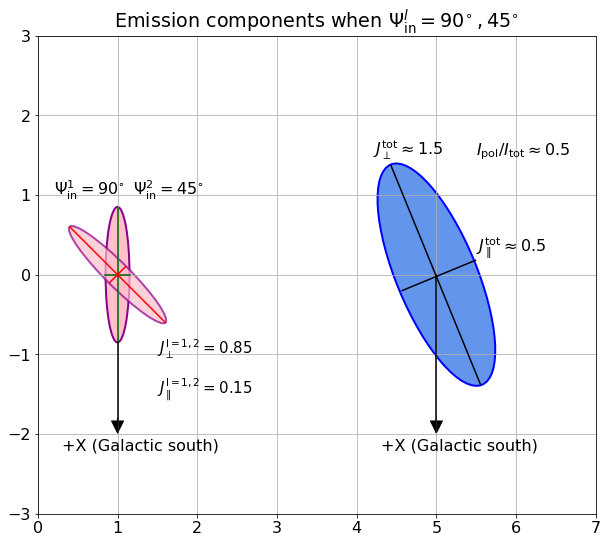
\includegraphics[width = 7cm]{Images/Pol_intensity_Ellipses_circles_emissions.png}
         \caption{Case II - Polarised intensity}
         \label{fig_pol_intensity}
     \end{subfigure}
     \hfill
    \caption{Simplified diagram of emission components for total and polarised intensities in terms of the polarisation ellipses.}
\end{figure}

\newpage
\section{Appendix B}\label{Appendix_B}
As discussed in section ~\ref{GMF} we generate the turbulent fields for our model using CRPropa3 ~\cite{CRPropa3_2016}. We the minimum and maximum wavelength we use to generate these fields are 
$L_{min}$ = 200 pc and $L_{max}$ = 400 pc and $L_{coh} \approx $~150 kpc. One of the major reasons why we do not have enough decades covered for the wavelength is because of the time it takes to generate these fields using CRPropa. 
We looked at power spectrum for different realisations of the turbulent field. In figure ~\ref{fig:PowerSpectrum} we plot power spectrum in X,Y and Z directions by averaging over the other two directions. We chose this particular realisation since it followed closely a power law spectrum of index (5/3). 
\begin{figure}[h!]
    \centering
    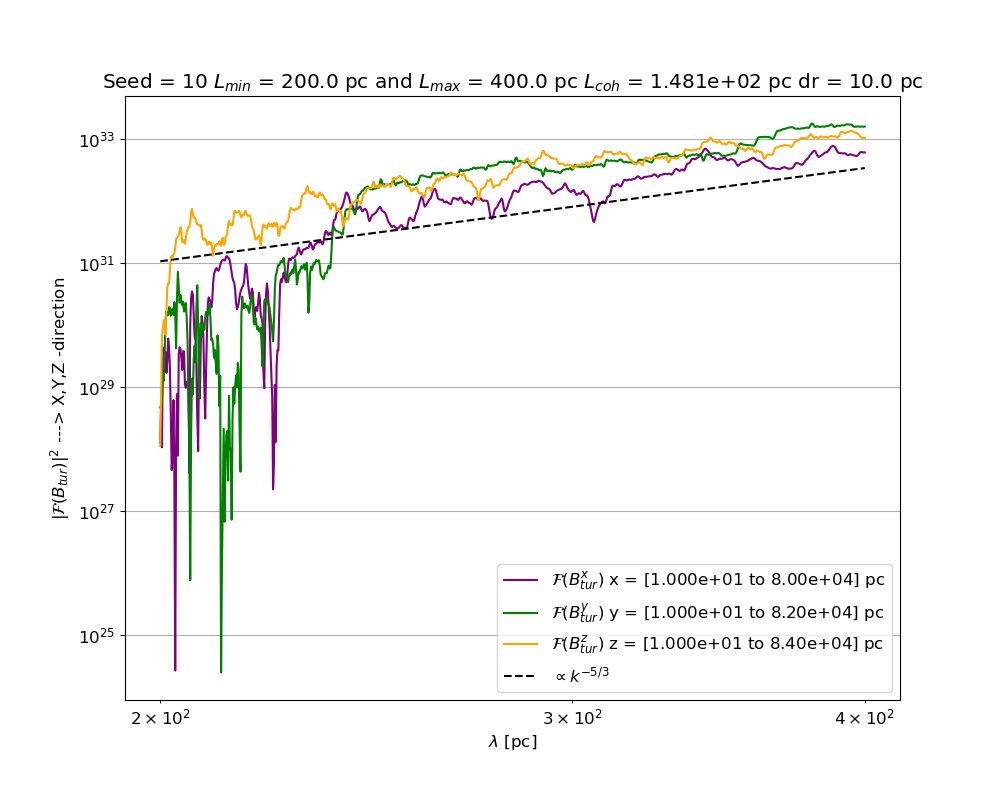
\includegraphics[width = 12cm]{Images/Jan3_Test_PowerSpectrum_vs_lambda_seed_10.png}
    \caption{Power spectrum plot versus wavelength for X, Y and Z direction.}
    \label{fig:PowerSpectrum}
\end{figure}
\section{Test skymap for arrival directions for the same source!}

\subsection{Arrival directions from sources on a grid for 30EeV and proton}

\iffalse

\newgeometry{top=20mm, bottom=20mm,lmargin=1.mm,rmargin=1.mm} 
\begin{figure}[h!]
    \centering
    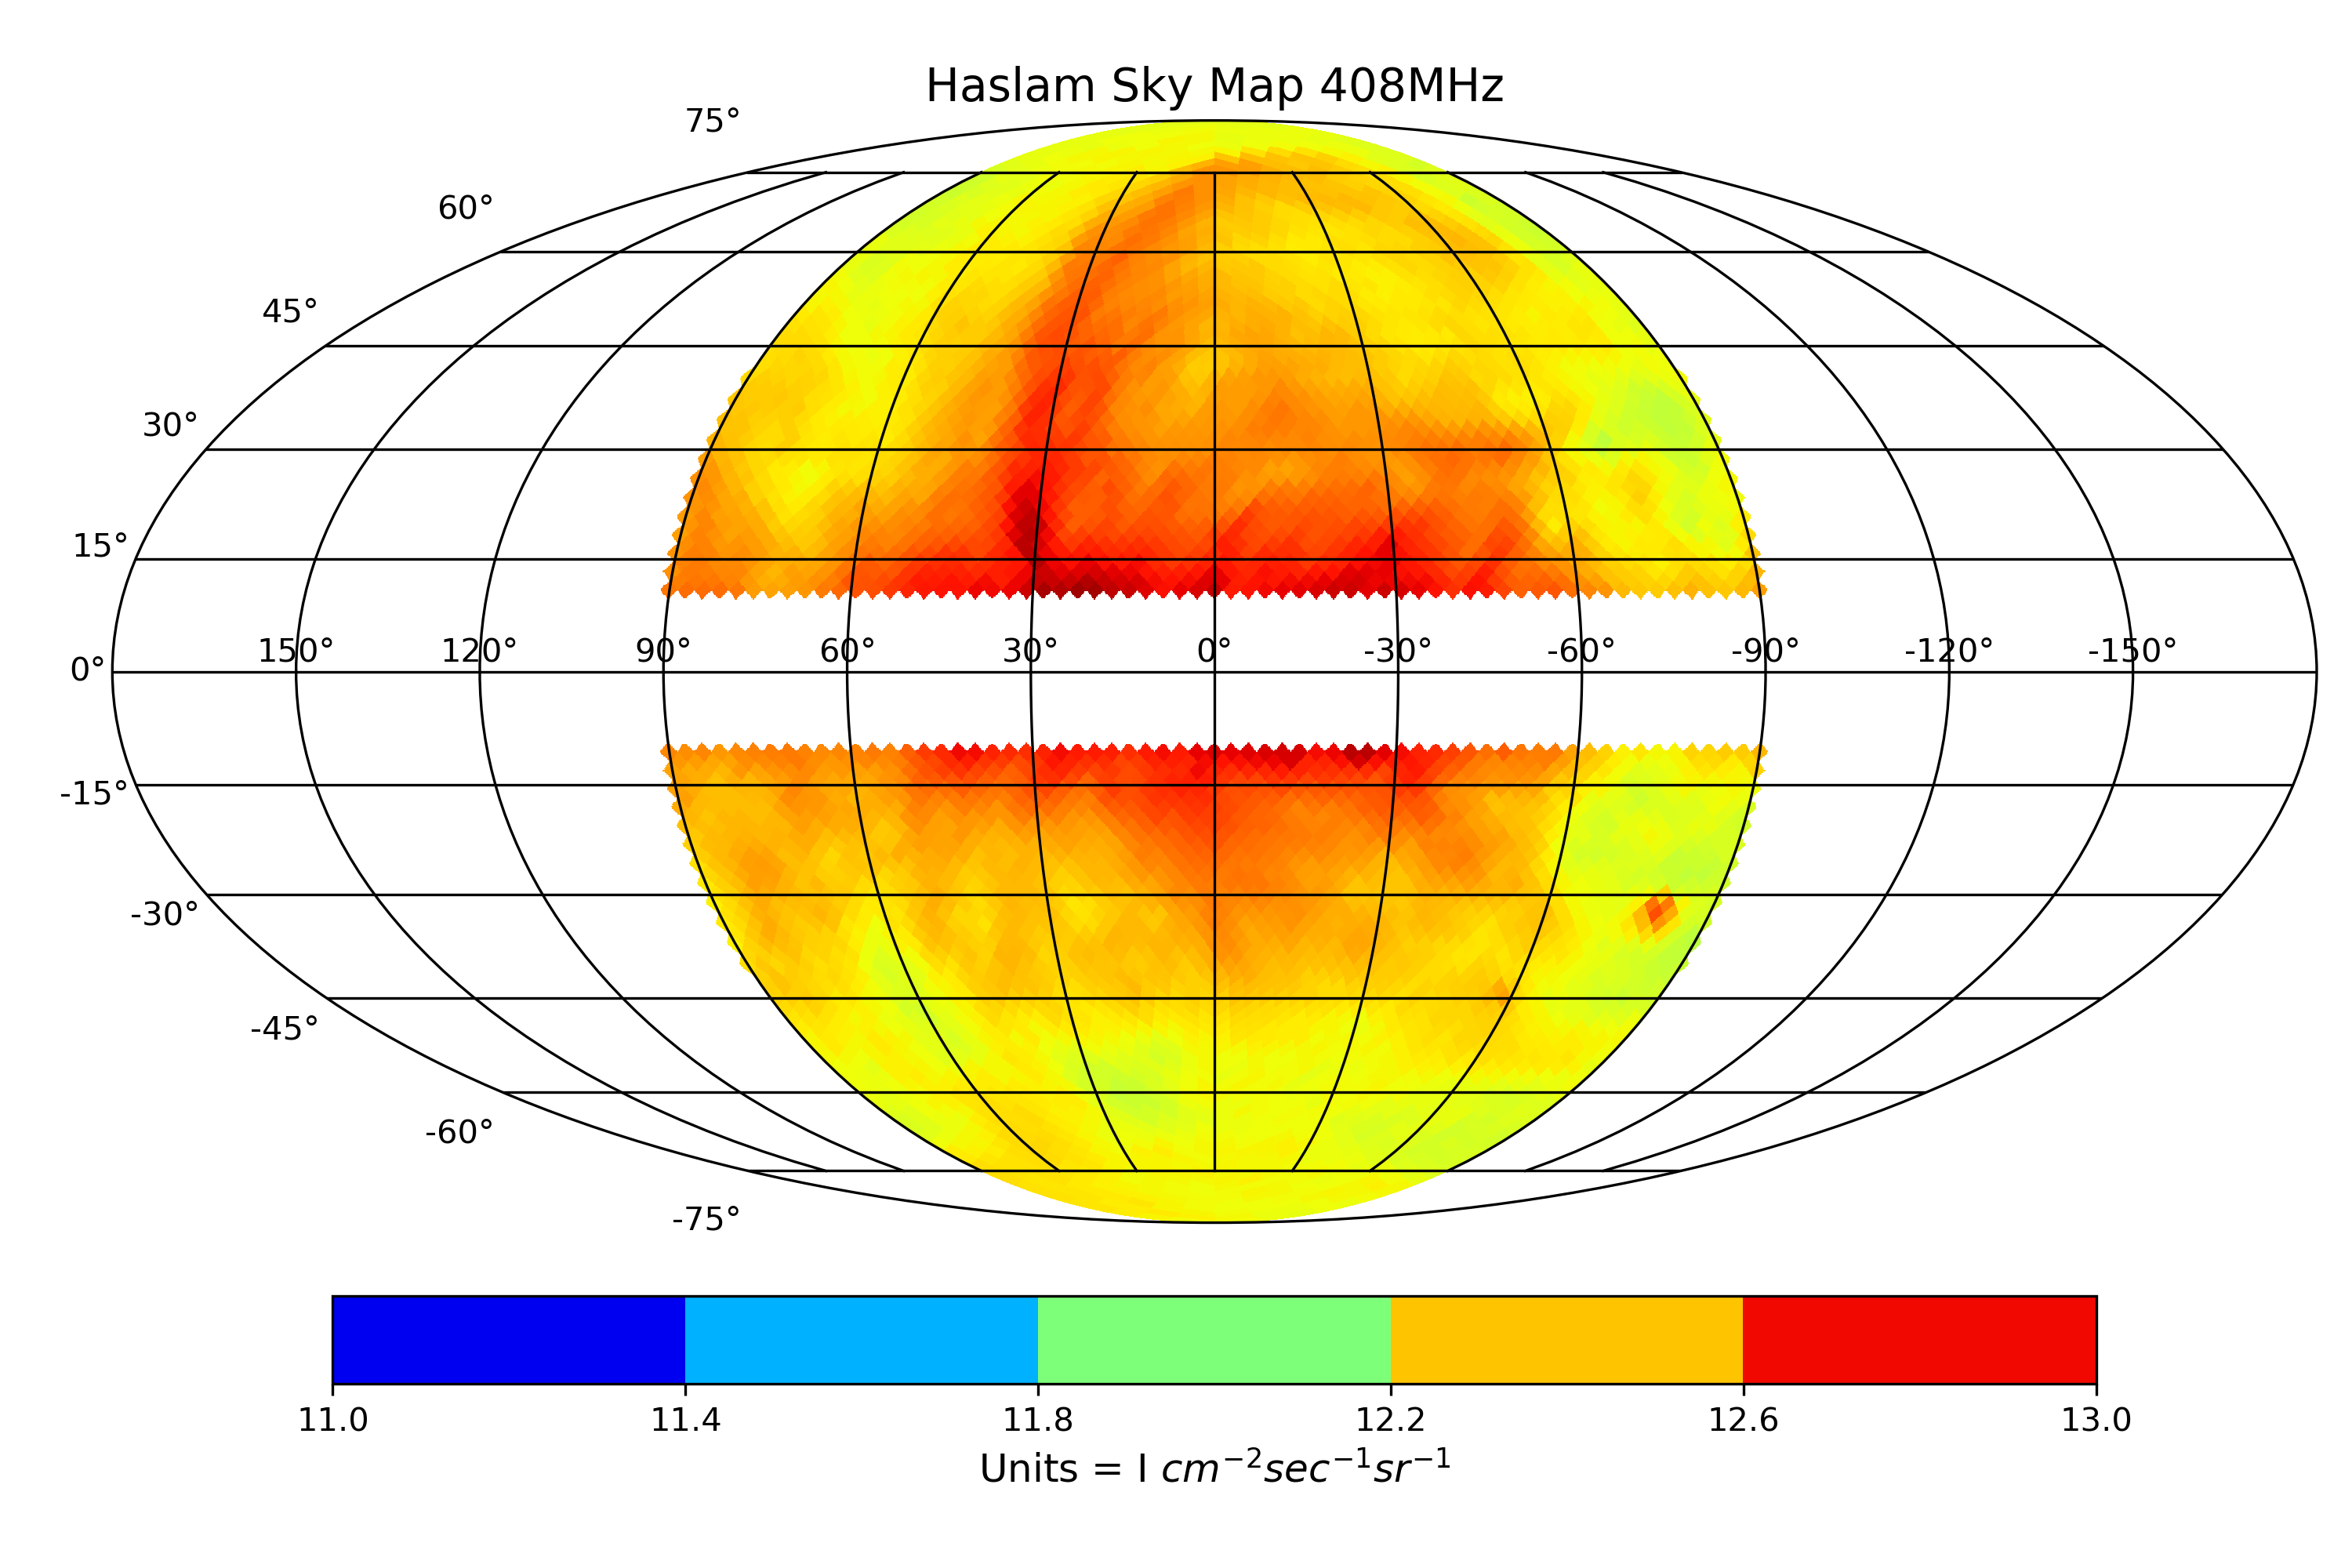
\includegraphics[width = 10cm]{Images/Haslam_408MHz.png}
    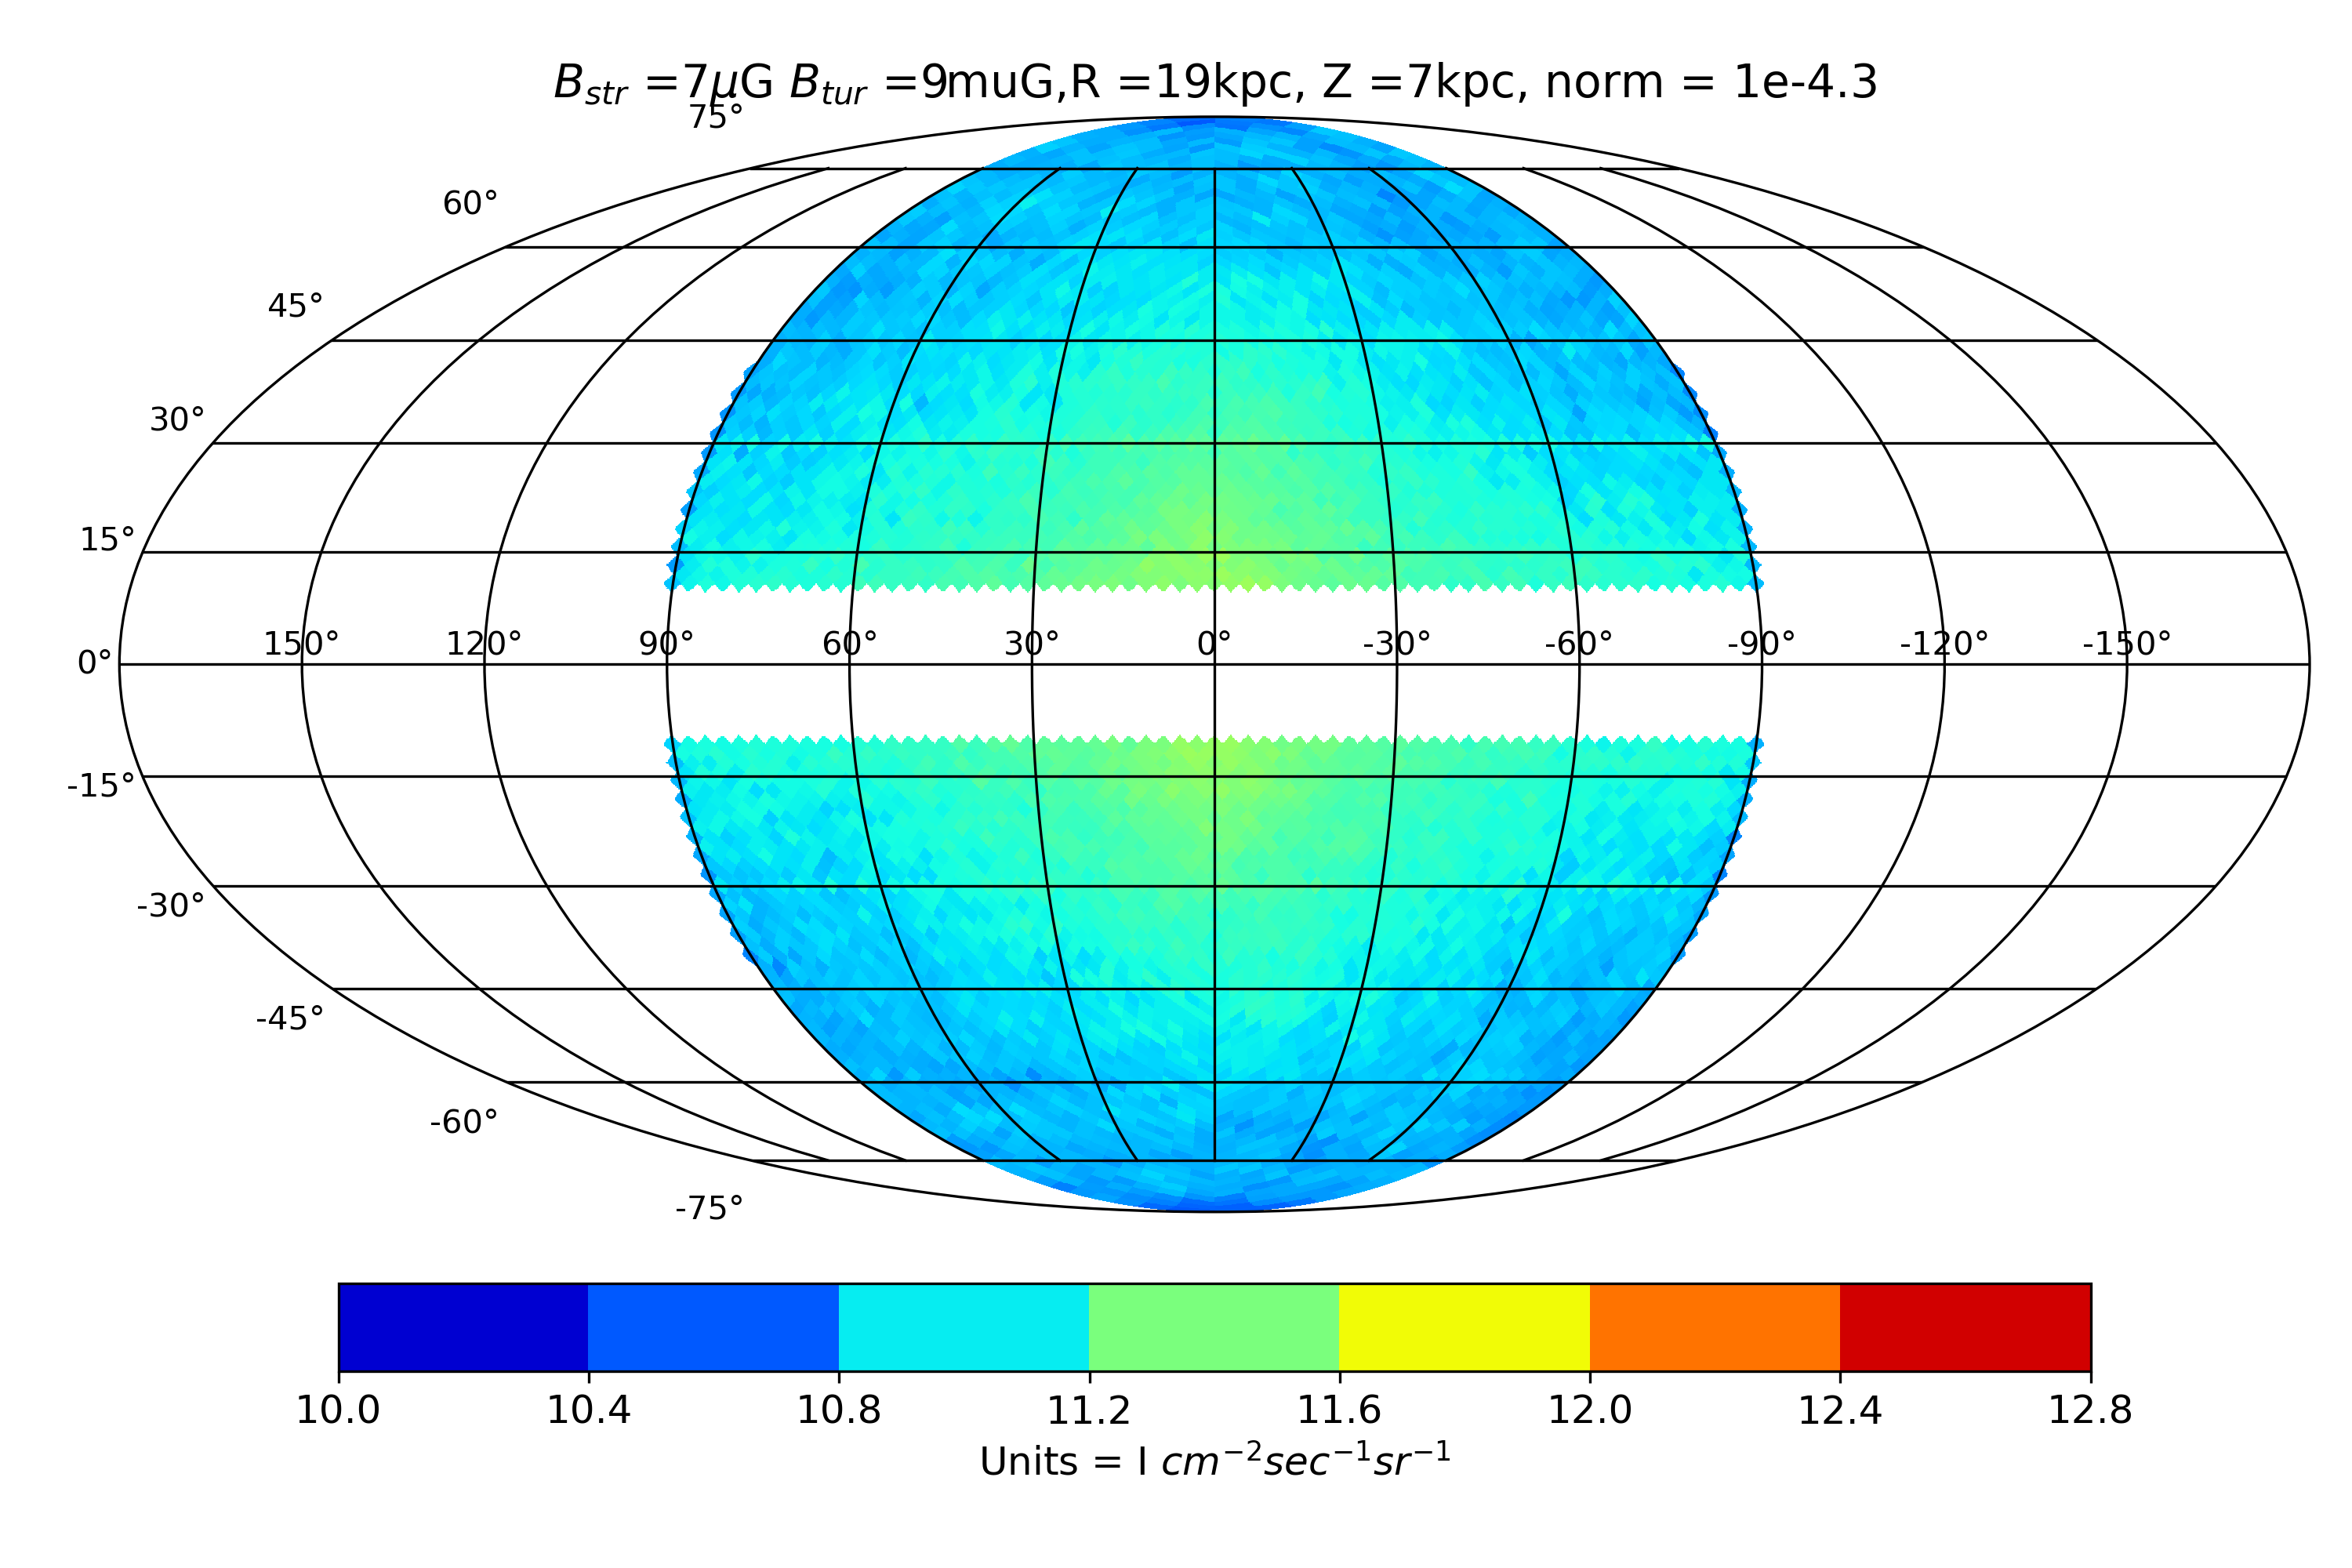
\includegraphics[width =
    10cm]{Images/408MHz_TI_Spec_Ind_3.0_Bstr_7_Btur_9_R_19_Z_7_norm_4.3.png}
 %   \includegraphics[width = 10cm]{Images/408MHz_TI_Spec_Ind_3.3_Bstr_5_Btur_10_R_12_Z_7.png}
    \caption{In figure Haslam data is shown top left, toy model total intensity map top right and in the bottom JF12 skymaps. The disc field is removed from this skymap and it includes Xfield, toroidal halo and turbulent fields.All calculated at $408$MHz. \Andrew{Color bar scales should have a fixed ranged (to allow easy comparison between maps)}}
    \label{fig:my_label}
\end{figure}
\newpage

\fi
\iffalse

\subsubsection{Faraday Rotation}\label{Faraday_Rotation}
The polarisation angle of an EM wave gets rotated by when passing through a magnetised plasma. The observed polarisation angle $\Psi_{\rm obs }$ is then a result of this rotation angle, $\Theta_{\rm RM} = RM\lambda^2$ and the intrinsic polarisation angle $\Psi_{\rm in}$. Here, $\lambda$ is the wavelength of the radiation and $RM \propto \int_0^L {\rm d}l(n_e B_{\parallel})$ is the rotation measure with $n_e$ being thermal electron density and $B_{\parallel}$ being the parallel component of magnetic field.

Hence, there is a need to calculate this new polarisation angle at each point along the line of sight in order to calculate $Q^l$ and $U^l$.\\ Below, is the value of polarisation angle at a point $l$ along the line of sight. $\Psi^l_{\rm obs}$ is the sum of the intrinsic polarisation $\Psi^l_{\rm in}$ and the effect of rotation measure ($\Theta_{\rm RM}$)up until the point in $l$.
\begin{eqnarray}
\Psi^l_{\rm obs} = \Psi^l_{\rm in} + \lambda^2  k_0\int_{0}^{l}  \rm{d}l \ n_e B_{\parallel}
\end{eqnarray}
here,$k_0 = 8.12 \ 1e3$ (in SI units \cite{Longair}) is a constant.
Equations for Stokes parameters will change from $Q^l_{\rm obs}$ \& $U^l_{\rm obs}$ will be dependant on the new polarisation angle $\Psi^l_{\rm obs}$. The new equation will be:
\begin{eqnarray}
Q^l_{\rm obs} = ({J_{\perp}^l} - {J_{\parallel}^l}) \ {\cos}(2\Psi^l_{\rm obs})
\end{eqnarray}
\begin{eqnarray}
U^l_{\rm obs} = ({J_{\perp}^l}- {J_{\parallel}}^l) \ {\sin}(2\Psi^l_{\rm obs}) \ .
\end{eqnarray}

This will also change the resultant observed polarised intensity $I_{\rm pol}^{\rm obs}$.
The new polarised intensity will be then:
\begin{eqnarray}
I_{\rm pol}^{\rm obs} = \sqrt{(\int_0^L \mathrm{d}l \ {Q^l}_{\rm obs})^2+(\int_0^L \ \mathrm{d}l \ {U^l_{\rm obs})^2}} \ .
\end{eqnarray}
\begin{figure}[h!]
    \centering
    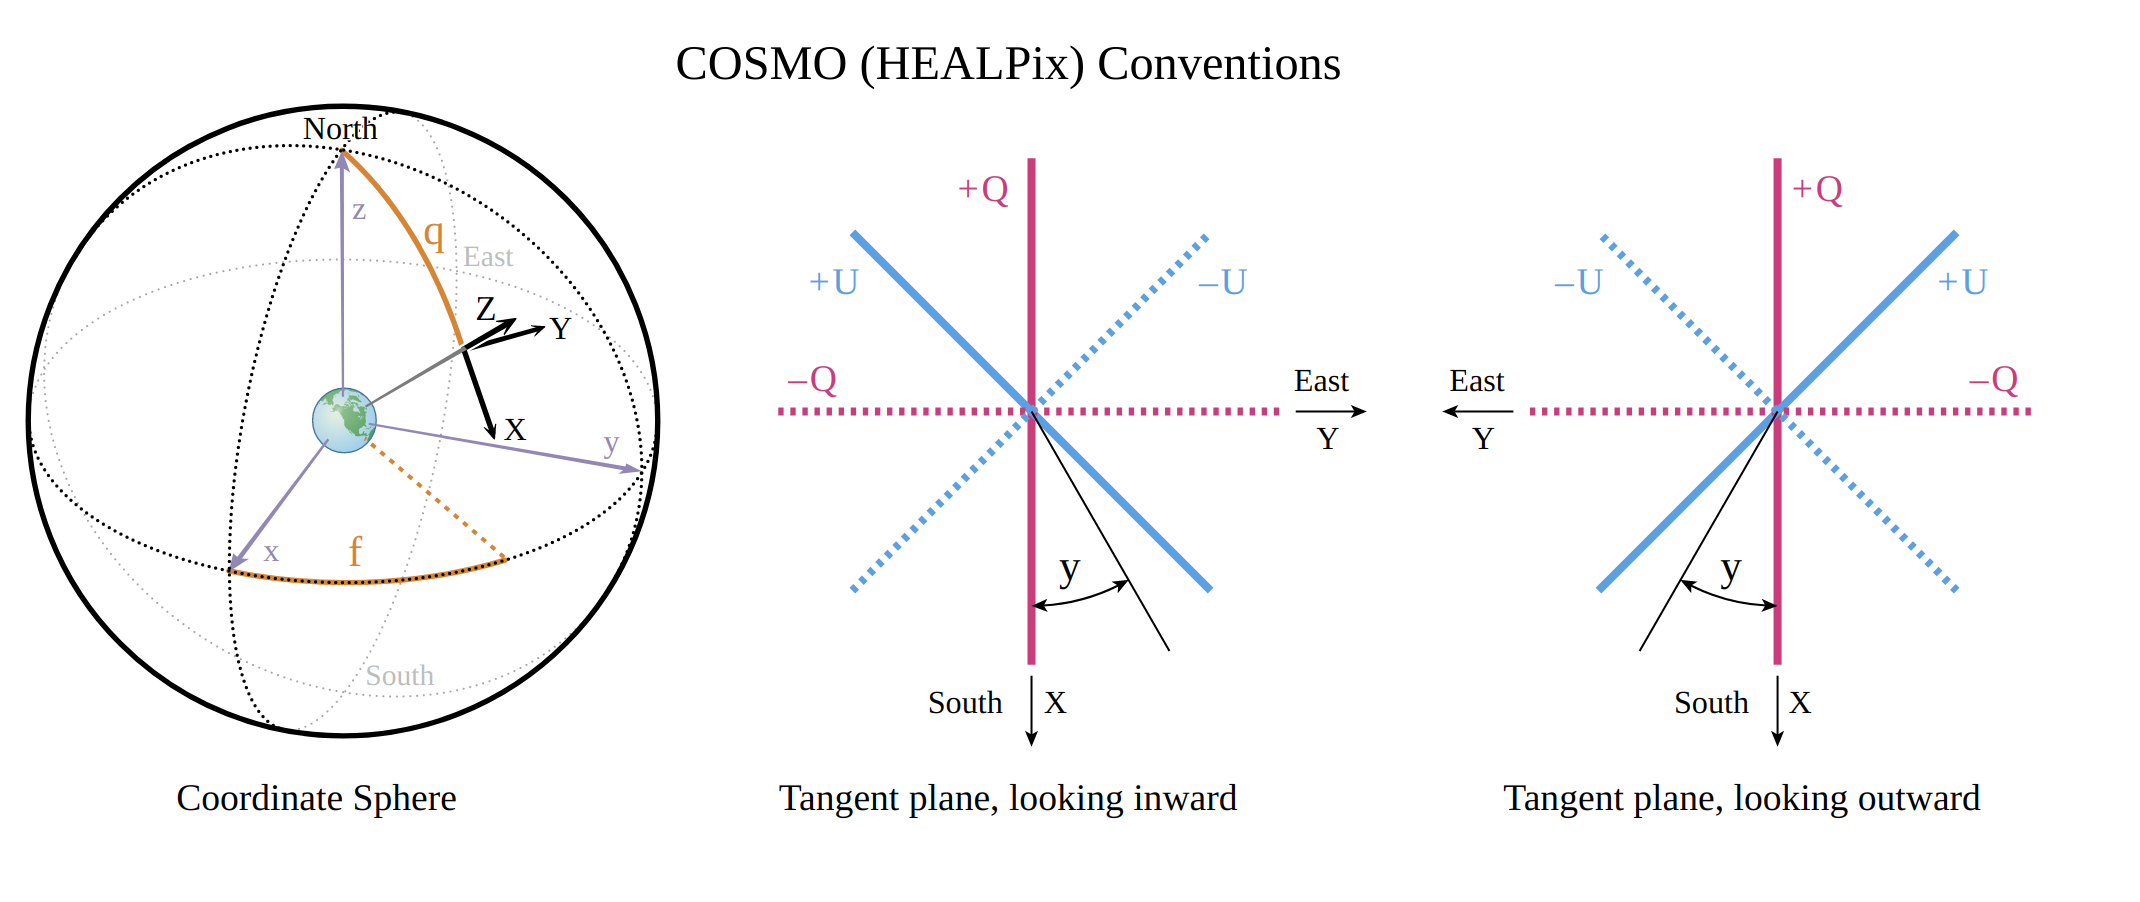
\includegraphics[width = 15cm]{Images/Healpix_Conventions.png}
    \caption{Healpix convention for the polarisation adopted by Planck which is also used for our calculations for better comparison of toy model data and observation data.}
    \label{fig:Planck_ang_con}
\end{figure}
\fi

\end{document}
